\section{Vektory}\label{sec:vectors}

\textbf{Vektor} je základním geometrickým objektem, který reprezentuje směr a velikost v prostoru.
Vektory se často používají k popisu pohybu, síly, rychlosti a dalších fyzikálních veličin, 
ale také k reprezentaci geometrických objektů a operací v analytické geometrii.
Na rozdíl od bodu, který určuje polohu, vektor popisuje posunutí mezi dvěma body.
Vektory označujeme $\vec{v}$, nebo $\mathbf{v}$. 

Nejprve si připomeneme co to je orientovaná úsečka (viz Obrázek \ref{fig:oriented_segment}).
\begin{definition}\label{def:oriented_segment}
    Orientovanou úsečkou rozumíme úsečku, která má určený směr od jednoho koncového bodu k druhému.    
\end{definition}

Na Obrázku~\ref{fig:oriented_segment} je znázorněna orientovaná úsečka určená body $A$ a $B$.
Velikost orientované úsečky $\overrightarrow{AB}$ je dána vzdáleností mezi body $A$ a $B$, 
tedy délkou úsečky $AB$. Směr orientované úsečky $\overrightarrow{AB}$ je určen směrem od bodu $A$ k bodu $B$.


\begin{figure}[H]
    \centering
    \begin{tikzpicture}
        \draw[vector] (0,0) -- (2,1);
        \node[below] at (0,0) {$A$};
        \node[below] at (2,1) {$B$};
    \end{tikzpicture}
    \caption{Vektor $\vec{v}$ určený body $A$ a $B$}
    \label{fig:oriented_segment}
\end{figure}

Zvláštním případem orientované úsečky je situace, kdy počáteční a koncový bod jsou totožné, tedy $A = B$.
V tomto případě mluvíme o \textbf{nulové orientované úsečce}. 
Její směr není určen, protože nelze rozlišit mezi počátečníma a koncovým bodem.
Její velikost je nulová.

\begin{remark}
Nulová orientovaná úsečka bude později odpovídat \textbf{nulovému vektoru}.
Ten hraje v počtu s vektory podobnou roli, jakou hraje číslo nula v aritmetice.
\end{remark}

Nyní můžeme formálně definovat vektor jako:

\begin{definition}\label{def:vector}
    \textbf{Vektorem} rozumíme orientovanou úsečku, která je určena počátečním a koncovým bodem.
\end{definition}

Vektory poté rozlišujeme podle jejich bodů určení, tedy podle počátečního a koncového bodu.

\begin{definition}\label{def:nonzero_vector}
    \textbf{Nenulový vektor} je množina všech orientovaných úseček, které mají stejnou velikost a směr, 
    ale mohou být určeny různými počátečními a koncovými body.
\end{definition}

\begin{definition}\label{def:zero_vector}
    \textbf{Nulový vektor} je množina všech nulových orientovaných úseček.
\end{definition}

\begin{example}\label{exa:oriented_segments}
    Na Obrázku~\ref{fig:oriented_segments} jsou znázorněny různé orientované úsečky, rozhodni které z nich jsou totožné vektory.
    \begin{figure}[H]
        \centering
        \begin{tikzpicture}[scale=1.1]

            % OP
            \draw[vector] (0,5) -- (3,5);
            \draw[thick] (0,4.85) -- (0,5.15);
            \node[below left] at (0,5) {$O$};
            \node[below right] at (3,5) {$P$};

            % EF
            \draw[vector] (-0.3,2.4) -- (2.2,4.0);
            \draw[thick] (-0.2,2.25) -- (-0.4,2.55);
            \node[below left] at (-0.3,2.4) {$E$};
            \node[above right] at (2.2,4.0) {$F$};

            % GH
            \draw[vector] (5.8,4.0) -- (4.3,3.0);
            \draw[thick] (5.7,4.15) -- (5.9,3.85);
            \node[below left] at (4.3,3.0) {$G$};
            \node[above right] at (5.8,4.0) {$H$};

            % IJ
            \draw[vector] (2.0,2.0) -- (5.5,2.0);
            \draw[thick] (2.0,1.85) -- (2.0,2.15);
            \node[below left] at (2.0,2.0) {$I$};
            \node[below right] at (5.5,2.0) {$J$};

            % AB
            \draw[vector] (6.2,1.0) -- (9.7,3.2);
            \draw[thick] (6.3,0.85) -- (6.1,1.15);
            \node[below left] at (6.2,1.0) {$A$};
            \node[above right] at (9.7,3.2) {$B$};

            % CD
            \draw[vector] (8.2,0.9) -- (12.0,0.9);
            \draw[thick] (8.2,0.75) -- (8.2,1.05);
            \node[below left] at (8.2,0.9) {$C$};
            \node[below right] at (12.0,0.9) {$D$};

            % KL
            \draw[vector] (11.0,5.5) -- (8.3,3.8);
            \draw[thick] (11.1,5.35) -- (10.9,5.65);
            \node[below left] at (8.3,3.8) {$K$};
            \node[above right] at (11.0,5.5) {$L$};

            % MN
            \draw[vector] (7.8,4.3) -- (9.2,5.1);
            \draw[thick] (7.9,4.15) -- (7.7,4.45);
            \node[below left] at (7.8,4.3) {$M$};
            \node[above right] at (9.2,5.1) {$N$};

        \end{tikzpicture}

        \begin{tabular}{ll}
            vektor $\vec{u}:$ &jsou orientované úsečky $\overrightarrow{AB}$, $\overrightarrow{EF}$ \\
            vektor $\vec{v}:$ &jsou orientované úsečky $\overrightarrow{CD}$, $\overrightarrow{IJ}$, $\overrightarrow{OP}$ \\
            vektor $\vec{w}:$ &je orientovaná úsečka $\overrightarrow{LK}$ \\
            vektor $\vec{x}:$ &je orientovaná úsečka $\overrightarrow{HG}$ \\
            vektor $\vec{y}:$ &je orientovaná úsečka $\overrightarrow{MN}$ \\            
        \end{tabular}
        \caption{Znázornění orientovaných úseček}
        \label{fig:oriented_segments}
    \end{figure}
\end{example}


\subsection{Vektory v kartézské soustavě souřadnic}\label{subsec:Vectors_in_cartesian_coordinate_system} 
\subsubsection{Souřadnice vektoru v rovině}\label{subsubsec:Coordinates_of_vector_in_plane}

Dosud jsme vektor chápali jako orientovanou úsečku.
V analytické geometrii však potřebujeme vektory vyjadřovat pomocí souřadnic.

Nechť $A = [x_1; y_1]$ a $B = [x_2; y_2]$ jsou dva body v rovině.

\begin{definition}\label{def:vector_coordinates}
    Vektor $\overrightarrow{AB}$ má souřadnice dané vztahem
    \begin{equation}\label{eq:vector_coordinates}
        \vec{v} = \overrightarrow{AB} = B - A = (x_2 - x_1;\, y_2 - y_1).
    \end{equation}
\end{definition}

\begin{remark}
    Souřadnice vektoru vyjadřují změnu souřadnic mezi počátečním a koncovým bodem,
    tedy „o kolik“ se musíme posunout ve směru osy $x$ a $y$.
\end{remark}

\begin{example}\label{exa:vector_coordinates}
    Nechť $A = [1; 2]$ a $B = [4; 6]$ jsou dva body v rovině.
    Souřadnice vektorů $\overrightarrow{AB}$ a $\overrightarrow{BA}$ určíme pomocí vztahu~\eqref{eq:vector_coordinates}:
    \[
    \vec{v} = \overrightarrow{AB} = B - A = (4 - 1;\, 6 - 2) = (3; 4).
    \]
    Tedy vektor $\overrightarrow{AB}$ má souřadnice $(3; 4)$.
    Pro vektor $\overrightarrow{BA}$ máme:
    \[
    \vec{v} = \overrightarrow{BA} = A - B = (1 - 4;\, 2 - 6) = (-3; -4).
    \]
    Tedy vektor $\overrightarrow{BA}$ má souřadnice $(-3; -4)$.
    \begin{figure}[H]
        \centering
        \begin{tikzpicture}
            \draw[vector] (-4,0) -- (-2,4) node[midway, above, sloped] {$\overrightarrow{AB}$};
            \node[below] at (-4,0) {$A$};
            \node[above] at (-2,4) {$B$};

            \draw[vector] (3,4) -- (1,0) node[midway, above, sloped] {$\overrightarrow{BA}$};
            \node[below] at (1,0) {$A$};
            \node[above] at (3,4) {$B$};
        \end{tikzpicture}
        \caption{Vektory $\overrightarrow{AB}$ a $\overrightarrow{BA}$}
        \label{fig:vector_coordinates_example}
    \end{figure}
\end{example}

Z příkladu~\ref{exa:vector_coordinates} (viz Obrázek~\ref{fig:vector_coordinates_example}) vidíme,
že vektory $\overrightarrow{AB}$ a $\overrightarrow{BA}$ mají stejnou velikost, ale opačný směr.

\begin{example}
    Je dán vektor $\vec{v} = (2; -1)$ a bod $A = [3; 4]$.
    Určete souřadnice bodu $B$, pro který platí $\vec{v} = \overrightarrow{AB}$.

    Použijeme vztah~\eqref{eq:vector_coordinates} pro vektor $\overrightarrow{AB}$:
    \[
    (2; -1) = B - A = (x_B - x_A; y_B - y_A).
    \]
    Dosadíme souřadnice bodu $A$ a dostaneme soustavu rovnic:
    \[
    \begin{cases}
        x_B - 3 = 2 \\
        y_B - 4 = -1
    \end{cases}
    \]
    Řešením této soustavy je $x_B = 5$ a $y_B = 3$.
    Tedy souřadnice bodu $B$ jsou $[5; 3]$.
\end{example}

\subsection{Operace s vektory v rovině}\label{subsec:Vector_operations_in_plane}

V předchozí části jsme si ukázali, jak vektor popisuje posunutí mezi dvěma body.
Abychom s vektory mohli dále pracovat, potřebujeme zavést základní operace,
které nám umožní tato posunutí kombinovat a upravovat.

Operace s vektory mají přirozený geometrický význam:
umožňují popsat skládání pohybů, změnu směru i změnu velikosti.
Zároveň je lze jednoduše vyjádřit pomocí souřadnic,
což z nich činí velmi účinný nástroj analytické geometrie.

Operace s vektory budou klíčové například při popisu přímek,
rovinných útvarů nebo při výpočtu úhlů mezi objekty.


\subsubsection{Velikost vektoru}\label{subsubsec:Vector_magnitude}
Nejprve si definujeme velikost vektoru, která nám umožní měřit délku orientované úsečky reprezentující vektor.

\begin{definition}
    \textbf{Velikost vektoru} $\vec{v} = (v_x; v_y)$ je dána vztahem
    \begin{equation}\label{eq:vector_magnitude}
        |\vec{v}| = \sqrt{v_x^2 + v_y^2}.
    \end{equation}
\end{definition}
Velikost vektoru odpovídá délce orientované úsečky, která reprezentuje tento vektor.
Tato délka vychází z \textbf{Pythagorovy věty} pro pravoúhlý trojúhelník, jehož odvěsnami jsou souřadnice vektoru $v_x$ a $v_y$ (viz Obrázek~\ref{fig:vector_magnitude_example}).
Velikost vektoru je vždy nezáporné reálné číslo, a nulový vektor má velikost rovnu nule.

\begin{figure}[H]
    \centering
    \begin{tikzpicture}
        % Osy
        \draw[<->, thick] (-1,0) -- (4,0) node[right] {$x$};
        \draw[<->, thick] (0,-1) -- (0,3) node[above] {$y$};

        % vektor v
        \draw[vector] (1,1.5) -- (3,2.5) node[midway, above, sloped] {$|\vec{v}|$};

        % pomocné čáry pro v_x a v_y
        \draw[dashed] (1,1.5) -- (3,1.5);
        \draw[dashed] (3,1.5) -- (3,2.5);
        \node[below] at (2,1) {$v_x ^2$};
        \node[right] at (3.2,2) {$v_y ^2$};

        % pythagorova věta pro velikost vektoru
        \draw[dashed] (1,1.5) -- (1,-0.5) -- (3,-0.5) -- (3,1.5);
        \draw[dashed] (3,1.5) -- (4,1.5) -- (4,2.5) -- (3,2.5);

        % čtverec nad přeponou
        \draw[dashed] (1,1.5) -- (0,3.25) -- (2,4.25) -- (3,2.5) -- cycle;
        \node[rotate=26] at (1.4,3) {$v_x^2 + v_y^2$};


    \end{tikzpicture}
    \caption{Velikost vektoru $\vec{v}$}
    \label{fig:vector_magnitude_example}
\end{figure}





Mějme vektory $\vec{u} = (u_x; u_y)$ a $\vec{v} = (v_x; v_y)$ v rovině.

\begin{figure}[H]
    \centering
    \begin{tikzpicture}
        \draw[vector] (-5,0) -- (-4,2);
        \node[left] at (-4.5,1) {$\vec{v}$};
        
        % vektor u
        \draw[vector] (-4.5,-1) -- (-1.5,0);
        \node[below] at (-3.2,-0.7) {$\vec{u}$};

    \end{tikzpicture}
    \caption{Vektory $\vec{u}$ a $\vec{v}$ v rovině}
    \label{fig:vector_operations_example}
\end{figure}


\subsubsection{Součet vektorů}\label{subsubsec:Vector_addition}
\begin{definition}\label{def:vector_addition}
    \textbf{Součet} vektorů $\vec{u}$ a $\vec{v}$ je vektor daný vztahem
    \begin{equation}\label{eq:vector_addition}
        \vec{u} + \vec{v} = (u_x + v_x;\, u_y + v_y).
    \end{equation}
\end{definition}

Geometricky lze součet vektorů $\vec{u}$ a $\vec{v}$ znázornit pomocí tzv. \textbf{paralelogramového pravidla}, neboli skládání vektorů do rovnoběžníku.
Podle paralelogramového pravidla umístíme oba vektory tak, aby měly společný počátek, a poté dokončíme paralelogram, jehož dvě strany jsou dané vektory.
Součet vektorů $\vec{u} + \vec{v}$ je pak vektor, který vede z počátku do protilehlého vrcholu tohoto paralelogramu.

\begin{figure}[H]
    \centering
    \begin{tikzpicture}
        % --- LEVÁ ČÁST ---
        % vektor v
        \draw[vector] (-5,0) -- (-4,2);
        \node[left] at (-4.5,1) {$\vec{v}$};
        
        % vektor u
        \draw[vector] (-4.5,-1) -- (-1.5,0);
        \node[below] at (-3.2,-0.7) {$\vec{u}$};
        
        % plus
        \node at (-3.5,0.5) {$+$};
        
        % rovná se
        \node at (-0.5,0.5) {$=$};
        
        % --- PRAVÁ ČÁST ---
        % počátek
        \coordinate (A) at (1,0);
        \node[below left] at (A) {$A$};
        
        % vektor u (z A)
        \draw[vector] (A) -- (4,1);
        \node[below] at (2,0.3) {$\vec{u}$};
        
        % vektor v (z A)
        \draw[vector] (A) -- (2,2);
        \node[left] at (0.7,1.2) {$\vec{v}$};
        
        % posunutý vektor v (od konce u)
        \draw[vector, gray] (4,1) -- (5,3);
        
        % posunutý vektor u (od konce v)
        \draw[vector, gray] (2,2) -- (5,3);
        
        % výsledný vektor
        \draw[vector] (A) -- (5,3) node[midway, above, sloped] {$\vec{v} + \vec{u}$};
    \end{tikzpicture}
    \caption{Sčítání vektorů (paralelogramové pravidlo)}
\end{figure}

\subsubsection{Rozdíl vektorů}\label{subsubsec:Vector_subtraction}
\begin{definition}\label{def:vector_subtraction}
    \textbf{Rozdíl} vektorů $\vec{u}$ a $\vec{v}$ je vektor daný vztahem
    \begin{equation}\label{eq:vector_subtraction}
        \vec{u} - \vec{v} = (u_x - v_x;\, u_y - v_y).
    \end{equation}
\end{definition}

Geometricky lze rozdíl vektorů $\vec{u}$ a $\vec{v}$ znázornit jako součet vektoru $\vec{u}$ a opačného vektoru $-\vec{v}$, který má stejnou velikost jako $\vec{v}$, ale opačný směr.
Podle paralelogramového pravidla umístíme vektor $\vec{u}$ a vektor $-\vec{v}$ tak, aby měly společný počátek, a poté dokončíme paralelogram, jehož dvě strany jsou dané vektory.
Rozdíl vektorů $\vec{u} - \vec{v}$ je pak vektor, který vede z počátku do protilehlého vrcholu tohoto paralelogramu.

\begin{figure}[H]
    \centering
    \begin{tikzpicture}
        % --- LEVÁ ČÁST ---
        % vektor v
        \draw[vector] (-5,0) -- (-4,2);
        \node[left] at (-4.5,1) {$\vec{v}$};
        
        % vektor u
        \draw[vector] (-4.5,-1) -- (-1.5,0);
        \node[below] at (-3.2,-0.7) {$\vec{u}$};
        
        % minus
        \node at (-3.5,0.5) {$-$};
        
        % rovná se
        \node at (-0.5,0.5) {$=$};


        % Paralelogramové pravidlo
        % počátek
        \coordinate (A) at (2,0);
        \node[below left] at (A) {$A$};

        % vektor u (z A)
        \draw[vector] (A) -- (5,1);
        \node[below] at (3.5,0.3) {$\vec{u}$};

        % vektor v (z A)
        \draw[vector] (A) -- (3,2);
        \node[left] at (2.5,1.2) {$\vec{v}$};

        % opačný vektor v k konce u
        \draw[vector, gray] (3,2) -- (0,1);

        % výsledný vektor
        \draw[vector] (A) -- (0,1) node[midway, above, sloped] {$\vec{v} - \vec{u}$};
    \end{tikzpicture}
    \caption{Znázornění rozdílu vektorů $\vec{v}$ a $\vec{u}$}
    \label{fig:vector_subtraction_example1}
\end{figure}

U odečítání vektorů je důležité si uvědomit, že rozdíl $\vec{u} - \vec{v}$ není totéž jako $\vec{v} - \vec{u}$, 
i přsto, že tyto dva vektory mají stejnou velikost, tak mají opačný směr.

\begin{figure}[H]
    \centering
    \begin{tikzpicture}
         % --- LEVÁ ČÁST ---
        % vektor v
        \draw[vector] (-5,0) -- (-4,2);
        \node[left] at (-4.5,1) {$\vec{v}$};
        
        % vektor u
        \draw[vector] (-4.5,-1) -- (-1.5,0);
        \node[below] at (-3.2,-0.7) {$\vec{u}$};
        
        % minus
        \node at (-3.5,0.5) {$-$};
        
        % rovná se
        \node at (-0.5,0.5) {$=$};


        % Paralelogramové pravidlo
        % počátek
        \coordinate (A) at (2,0);
        \node[below left] at (A) {$A$};

        % vektor u (z A)
        \draw[vector] (A) -- (5,1);
        \node[below] at (3.5,0.3) {$\vec{u}$};        

        % vektor v (z A)
        \draw[vector] (A) -- (3,2);
        \node[left] at (2.5,1.2) {$\vec{v}$};
        
        % opačný vektor v k konce u
        \draw[vector, gray] (5,1) -- (4,-1);

        % výsledný vektor
        \draw[vector] (A) -- (4,-1) node[midway, below, sloped] {$\vec{u} - \vec{v}$};

    \end{tikzpicture}
    
    \caption{Znázornění rozdílu vektorů $\vec{u}$ a $\vec{v}$}
    \label{fig:vector_subtraction_example2}
\end{figure}

A jak si můžeme všimnout z Obrázku~\ref{fig:vector_subtraction_example1} a Obrázku~\ref{fig:vector_subtraction_example2},
že vektory $\vec{u} - \vec{v}$ a $\vec{v} - \vec{u}$ mají stejnou velikost, ale opačný směr.
Platí tedy, že $\vec{u} - \vec{v} = -(\vec{v} - \vec{u})$.

\begin{example}
    Jsou dány vektory $\vec{u} = (3; 2)$ a $\vec{v} = (-1; 3)$. Určete souřadnice vektorů $\vec{w} = \vec{u} + \vec{v}$ a $\vec{x} = \vec{u} - \vec{v}$.
    Pro součet vektorů $\vec{w}$ použijeme vzorec~\eqref{eq:vector_addition}:
    \[
    \vec{w} = \vec{u} + \vec{v} = (3 + (-1); 2 + 3) = (2; 5).
    \]
    Pro rozdíl vektorů $\vec{x}$ použijeme vzorec~\eqref{eq:vector_subtraction}:
    \[
    \vec{x} = \vec{u} - \vec{v} = (3 - (-1); 2 - 3) = (4; -1).
    \]
    Tedy souřadnice vektoru $\vec{w}$ jsou $(2; 5)$ a souřadnice vektoru $\vec{x}$ jsou $(4; -1)$.
\end{example}

\begin{example}
    Je dán bod $A = [1; 2]$ a vektor $\vec{v} = (3; 4)$. 
    Určete souřadnice bodu $B$, pro který platí $\vec{v} = \overrightarrow{AB}$.
    Použijeme vztah~\eqref{eq:vector_coordinates} pro vektor $\overrightarrow{AB}$:
    \begin{align*}
        \vec{v} &= \overrightarrow{AB} \\
        \vec{v} & = B - A \\
        (v_x; v_y)  &= (x_B - x_A; y_B - y_A)
    \end{align*}

    Po dosazení souřadnic vektoru $\vec{v}$ a bodu $A$ dostaneme:
    \[
    (3;4) = (x_B - 1; y_B - 2)
    \]

    Tedy soustava rovnic pro souřadnice bodu $B$ je:
    \begin{align*}
        x_B - 1 &= 3 \\
        y_B - 2 &= 4
    \end{align*}
    Řešením této soustavy je $x_B = 4$ a $y_B = 6$.
    Tedy souřadnice bodu $B$ jsou $[4; 6]$.
\end{example}

Sčítání vektorů je komutativní a asociativní operace.
Pro odčítání tyto vlastnosti obecně neplatí.
Pro vektory $\vec{u}$, $\vec{v}$, $\vec{w}$ a $\vec{0}$ platí:
\begin{itemize}
    \item Komutativita sčítání: $\vec{u} + \vec{v} = \vec{v} + \vec{u}$,
    \item Asociativita sčítání: $(\vec{u} + \vec{v}) + \vec{w} = \vec{u} + (\vec{v} + \vec{w})$,
    \item Pro každý vektor $\vec{u}$ platí $\vec{u} + \vec{0} = \vec{u}$,
    \item Pro každý vektor $\vec{u}$ existuje opačný vektor $-\vec{u}$ tak, že $\vec{u} + (-\vec{u}) = \vec{0}$.
\end{itemize}


\begin{example}
    Je dán pravidelný šestiuhelník $ABCDEF$. Označte vektory $\vec{u} = C - A$, $\vec{v} = B - D$ a $\vec{w} = F - B$. 
    Určete výslednou souřadnici vektoru $\vec{u} + \vec{v} + \vec{w}$.
    
    Prvně ale využjme vlastnost, že vektor $\vec{u}$, který je dán orientovanou úsečkou $\overrightarrow{AC}$ je roven vektoru $\vec{u}$, který je dán orientovanou úsečkou $\overrightarrow{FD}$ (viz Obrázek~\ref{fig:vector_operations_hexagon}).
    
    \begin{figure}[H]
        \centering
        \begin{tikzpicture}
            \draw[thick] (0,0) coordinate[label=below:$A$] (A) 
            -- (2,0) coordinate[label=below:$B$] (B) 
            -- (3,1.73) coordinate[label=right:$C$] (C) 
            -- (2,3.46) coordinate[label=above:$D$] (D) 
            -- (0,3.46) coordinate[label=above:$E$] (E) 
            -- (-1,1.73) coordinate[label=left:$F$] (F) 
            -- cycle;

            \draw[vector, brown] (A) -- (C) node[midway, above, sloped] {$\vec{u}$};
            \draw[vector, gray] (D) -- (B) node[midway, above, sloped] {$\vec{v}$};
            \draw[vector, blue] (B) -- (F) node[midway, above, sloped] {$\vec{w}$};
            \draw[vector, dashed, brown] (F) -- (D) node[midway, above, sloped] {$\vec{u}$};
        \end{tikzpicture}
        \caption{Vektory $\vec{u}$, $\vec{v}$ a $\vec{w}$ v pravidelném šestiuhelníku}
        \label{fig:vector_operations_hexagon}
    \end{figure}

    Nyní můžeme použít vlastnosti sčítání vektorů a zjistit jejich výsledný součet.
    \begin{align*}
        \vec{u} + \vec{v} + \vec{w} &= \overrightarrow{FD} + \overrightarrow{DB} + \overrightarrow{BF} \\
                                    &= (D - F) + (B - D) + (F - B) \\
                                    &= D - F + B - D + F - B \\
                                    &= D - D + B - B + F - F \\
                                    &= 0 + 0 + 0 \\
                                    &= \vec{0}
    \end{align*}
   
    Vyšlo tedy, že součet vektorů $\vec{u} + \vec{v} + \vec{w}$ je roven nulovému vektoru $\vec{0}$, což znamená, že výsledný vektor nemá žádnou velikost ani směr.
    Toto můžeme zároveň geometricky interpretovat tak, že vektory $\vec{u}$, $\vec{v}$ a $\vec{w}$ tvoří uzavřenou smyčku, která se vrací zpět do výchozího bodu (viz Obrázek~\ref{fig:vector_operations_hexagon}).
\end{example}



\subsubsection{Násobení vektoru skalárem}\label{subsubsec:Vector_multiplication_by_scalar}

Doposud jsme vektory sčítali a odčítali.
Další základní operací je násobení vektoru \textbf{skalárem}, což je reálné číslo.

Tato operace nám umožňuje měnit velikost vektoru,
aniž bychom měnili jeho směr (v případě kladného čísla),
nebo směr obrátit (v případě záporného čísla).

\begin{definition}\label{def:scalar_multiplication}
    Nechť $\vec{v} = (v_x; v_y)$ je vektor a $k \in \mathbb{R}$.
    Násobení vektoru $\vec{v}$ číslem $k$ je dáno vztahem
    \begin{equation}\label{eq:scalar_multiplication}
        k \cdot \vec{v} = (k \cdot v_x;\, k \cdot v_y).
    \end{equation}
\end{definition}

\begin{remark}
    Násobení vektoru skalárem má následující geometrické důsledky:
    \begin{itemize}
        \item Pro $k > 0$ má vektor $k\vec{v}$ stejný směr jako $\vec{v}$.
        \item Pro $k < 0$ má vektor $k\vec{v}$ opačný směr než $\vec{v}$.
        \item Pro $k = 0$ platí $k\vec{v} = \vec{0}$.
    \end{itemize}
\end{remark}

\begin{figure}[H]
    \centering
    \begin{tikzpicture}

        % Osy
        \draw[<->, thick] (-3,0) -- (4.2,0) node[right] {$x$};
        \draw[<->, thick] (0,-3.7) -- (0,4.5) node[above] {$y$};

        % -------------------------
        % Vektor v
        % -------------------------
        \coordinate (A1) at (1.7,2.6);
        \coordinate (B1) at (3.3,3.5);

        \draw[vector] (A1) -- (B1);
        \node[above] at (2.3,3.1) {$\vec{v}$};

        % pomocné čáry pro p, q
        \draw[dashed] (A1) -- (3.3,2.6);
        \draw[dashed] (B1) -- (3.3,2.6);

        \node[below] at (2.5,2.6) {$p$};
        \node[right] at (3.3,3.05) {$q$};

        % -------------------------
        % Vektor 2v
        % -------------------------
        \coordinate (A2) at (-2.7,-1);
        \coordinate (B2) at (1.7,1.3);

        \draw[vector] (A2) -- (B2);
        \node[left] at (-0.4,0.5) {$2\vec{v}$};

        % pomocné čáry pro 2p, 2q
        \draw[dashed] (A2) -- (1.7,-1);
        \draw[dashed] (B2) -- (1.7,-1);

        \node[below] at (-0.4,-1) {$2p$};
        \node[right] at (1.7,0.4) {$2q$};

        % -------------------------
        % Vektor (-1)v
        % -------------------------
        \coordinate (A3) at (2.8,-1.6);
        \coordinate (B3) at (1.2,-2.5);

        \draw[vector] (A3) -- (B3);
        \node[above] at (2.0,-1.95) {$(-1)\vec{v}$};

        % pomocné čáry pro -p, -q
        \draw[dashed] (A3) -- (2.8,-2.5);
        \draw[dashed] (B3) -- (2.8,-2.5);

        \node[below] at (2.0,-2.5) {$-p$};
        \node[right] at (2.8,-2.05) {$-q$};

    \end{tikzpicture}
    \caption{Násobení vektoru skalárem}
    \label{fig:scalar_multiplication_vector}
\end{figure}

Z Obrázku~\ref{fig:scalar_multiplication_vector} vidíme, že násobením vektoru kladným číslem se jeho směr nemění, ale mění se jeho velikost. 
Naopak násobení číslem $-1$ zachová velikost vektoru, ale obrátí jeho směr.


\begin{example}
    Mějme $\vec{v} = (3; -4)$ a $k = 2$. 
    Určete velikost vektoru $\vec{v}$, souřadnice vektoru $k\vec{v}$ a velikost tohoto vektoru.

    Pro velikost vektoru $\vec{v}$ použijeme vzorec~\eqref{eq:vector_magnitude}:
    \[
    |\vec{v}| = \sqrt{3^2 + (-4)^2} = \sqrt{9 + 16} = \sqrt{25} = 5.
    \]

    Pro násobení vektoru $\vec{v}$ číslem $k$ použijeme vzorec~\eqref{eq:scalar_multiplication}:
    \[
    k\vec{v} = 2(3; -4) = (6; -8).
    \]

    Pro velikost vektoru $k\vec{v}$ opět použijeme vzorec~\eqref{eq:vector_magnitude}:
    \[
    |k\vec{v}| = \sqrt{6^2 + (-8)^2} = \sqrt{36 + 64} = \sqrt{100} = 10.
    \]

    Vidíme, že platí vztah
    \[
    |k\vec{v}| = |k| \cdot |\vec{v}|.
    \]

    Tedy souřadnice vektoru $k\vec{v}$ jsou $(6; -8)$ a jeho velikost je $10$.
\end{example}

\begin{example}
    Nechť $\vec{v} = (2; 3)$ a $k = -1$. Určete souřadnice vektoru $k\vec{v}$ a jeho velikost.

    Pro násobení vektoru $\vec{v}$ číslem $k$ použijeme vzorec~\eqref{eq:scalar_multiplication}:
    \[
    k\vec{v} = -1(2; 3) = (-2; -3).
    \]

    Pro velikost vektoru $k\vec{v}$ opět použijeme vzorec~\eqref{eq:vector_magnitude}:
    \[
    |k\vec{v}| = \sqrt{(-2)^2 + (-3)^2} = \sqrt{4 + 9} = \sqrt{13}.
    \]

    Tedy souřadnice vektoru $k\vec{v}$ jsou $(-2; -3)$ a jeho velikost je $\sqrt{13}$.
\end{example}

\begin{example}
    Nechť $\vec{v} = (1; -2)$ a $k = 0$. Určete souřadnice vektoru $k\vec{v}$ a jeho velikost.

    Pro násobení vektoru $\vec{v}$ číslem $k$ použijeme vzorec~\eqref{eq:scalar_multiplication}:
    \[
    k\vec{v} = 0(1; -2) = (0; 0).
    \]

    Pro velikost vektoru $k\vec{v}$ opět použijeme vzorec~\eqref{eq:vector_magnitude}:
    \[
    |k\vec{v}| = \sqrt{0^2 + 0^2} = \sqrt{0} = 0.
    \]

    Tedy souřadnice vektoru $k\vec{v}$ jsou $(0; 0)$ a jeho velikost je $0$.
\end{example}


\begin{definition}[Vlastnosti násobení vektoru skalárem]
    Pro každé dva vektory $\vec{u}$ a $\vec{v}$ a pro každá reálná čísla $k$ a $l$ platí následující vlastnosti:
    \begin{itemize}
        \item $\vec{0} \cdot \vec{u} = \vec{0}$,
        \item $-1 \cdot \vec{u} = -\vec{u}$,
        \item $k \cdot (\vec{u} + \vec{v}) = k \cdot \vec{u} + k \cdot \vec{v}$,
        \item $(k + l) \cdot \vec{u} = k \cdot \vec{u} + l \cdot \vec{u}$,
        \item $k \cdot (l \cdot \vec{u}) = (k \cdot l) \cdot \vec{u}$.
    \end{itemize}
\end{definition}


\subsection{Lineární kombinace}\label{subsec:Linear_combinations}

Pomocí sčítání vektorů a jejich násobení skalárem můžeme vytvářet nové vektory.
Tyto vektory nazýváme \textbf{lineární kombinace}.

\begin{definition}\label{def:linear_combination}
    Nechť $\vec{u}$ a $\vec{v}$ jsou vektory a $k, l \in \mathbb{R}$.
    Vektor tvaru
    \begin{equation}\label{eq:linear_combination}
        k\vec{u} + l\vec{v}
    \end{equation}
    nazýváme lineární kombinací vektorů $\vec{u}$ a $\vec{v}$.
\end{definition}

\begin{remark}
    Obecně můžeme lineární kombinaci definovat i pro více vektorů.

    Jsou-li dány vektory $\vec{u}_1, \vec{u}_2, \ldots, \vec{u}_n$ a reálná čísla $a_1, a_2, \ldots, a_n$,
    pak vektor
    \[
    \vec{v} = a_1 \vec{u}_1 + a_2 \vec{u}_2 + \cdots + a_n \vec{u}_n
    \]
    nazýváme \textbf{lineární kombinací} vektorů $\vec{u}_1, \vec{u}_2, \ldots, \vec{u}_n$.

    Reálná čísla $a_1, a_2, \ldots, a_n$ nazýváme \textbf{koeficienty lineární kombinace}.
\end{remark}

\begin{remark}
Lineární kombinace nám umožňují popsat, jak lze z daných vektorů „složit“ jiné vektory.
Měníme jejich velikost (násobením skalárem) a poté je sčítáme.

Lineární kombinace dvou vektorů $\vec{u}$ a $\vec{v}$ popisují všechny vektory,
které lze tímto způsobem získat.

Pokud vektory $\vec{u}$ a $\vec{v}$ nejsou rovnoběžné,
pak jejich lineární kombinace vyplňují celou rovinu.
\end{remark}

\begin{figure}[H]
    \centering
    \begin{tikzpicture}[scale=0.8]
         % --- LEVÁ ČÁST ---
        % vektor v
        \draw[vector] (-5,0) -- (-4.25,1.75);
        \node[left] at (-4.5,1) {$\vec{v}$};
        
        % vektor u
        \draw[vector] (-4.5,-1) -- (-1.5,0);
        \node[below] at (-3.2,-0.7) {$\vec{u}$};

        \draw[vector, gray] (-4.25,1.75) -- (-3.5,3.5);
        \draw[vector, gray] (-3.5,3.5) -- (-2.75,5.25);
        \node[left] at (-3.5,3) {$3\vec{v}$};

        % vektor 2u
        \draw[vector, gray] (-1.5,0) -- (1.5,1);
        \node[below] at (-2,0) {$2\vec{u}$};

        % rightarrow
        \node at (2,1.5) {$\Rightarrow$};

        % --- PRAVÁ ČÁST ---

        % vektor v
        \draw[vector] (-5+8,0) -- (-4.25+8,1.75);
        \node[left] at (-4.5+8,1) {$\vec{v}$};
        
        % vektor u
        \draw[vector] (-4.5+8-0.5,-1+1) -- (-1.5+8-0.5,0+1);
        \node[below] at (-3.2+8,-0.7+1) {$\vec{u}$};

        % vektor 3v
        \draw[vector, gray] (-4.25+8,1.75) -- (-3.5+8,3.5);
        \draw[vector, gray] (-3.5+8,3.5) -- (-2.75+8,5.25);
        \node[left] at (-3.5+8,3) {$3\vec{v}$};

        % vektor 2u
        \draw[vector, gray] (-1.5+8-0.5,0+1) -- (1.5+8-0.5,1+1);
        \node[below] at (-2+8-0.5,0+1) {$2\vec{u}$};

        % posunutý vektor 3v (od konce 2u)
        \draw[vector, gray] (1.5+8-0.5,1+1) -- (2.25+8-0.5,3.75);
        \draw[vector, gray] (2.25+8-0.5,3.75) -- (3+8-0.5,5.5);
        \draw[vector, gray] (3+8-0.5,5.5) -- (3.75+8-0.5,7.25);

        % posunutý vektor 2u (od konce 3v)
        \draw[vector, gray] (-2.75+8,5.25) -- (0.25+8,6.25);
        \draw[vector, gray] (0.25+8,6.25) -- (3.75+8-0.5,7.25);



        % vektor 2u + 3v
        \draw[vector, blue] (-5+8,0) -- (3.75+8-0.5,7.25);
        \node[above, rotate=42] at (0.375+6.5,3.625) {$2\vec{u} + 3\vec{v}$};
    \end{tikzpicture}
    \caption{Znázornění lineární kombinace $2\vec{u} + 3\vec{v}$}
    \label{fig:vector_linear_combination_example}
\end{figure}

\begin{example}
    Nechť $\vec{u} = (3;1)$ a $\vec{v} = (1;2)$.
    Určete lineární kombinaci $2\vec{u} + 3\vec{v}$.

    Prvně vypočítáme $2\vec{u}$ a $3\vec{v}$ pomocí vzorce~\eqref{eq:scalar_multiplication}:
    \[
    2\vec{u} = (6;2) \quad \text{a} \quad 3\vec{v} = (3;6).
    \]
    Nyní můžeme spočítat lineární kombinaci $2\vec{u} + 3\vec{v}$ pomocí vzorce~\eqref{eq:vector_addition}:    
    \[
    2\vec{u} + 3\vec{v} = (6;2) + (3;6) = (9;8).
    \]
    
    Výsledkem je vektor $(9;8)$, který představuje lineární kombinaci vektorů $\vec{u}$ a $\vec{v}$. (viz Obrázek~\ref{fig:vector_linear_combination_example}).
\end{example}

Pomocí lineárních kombinací dokážeme vytvářet nové vektory.
Někdy však potřebujeme určit vztah mezi dvěma konkrétními vektory,
například zda jsou na sebe kolmé nebo jaký úhel svírají.

K tomu slouží skalární součin.

\begin{remark}
Lineární kombinace nám umožňují vyjádřit jeden vektor pomocí jiných vektorů.
Tato myšlenka bude klíčová například při řešení soustav rovnic nebo při popisu přímek a rovin.
\end{remark}


\subsection{Skalární součin vektorů}\label{subsec:Dot_product_of_vectors}

V předchozí části jsme se naučili, jak s vektory počítat a jak měnit jejich velikost.
Často však potřebujeme určit vztah mezi dvěma vektory, například zda jsou na sebe kolmé,
nebo jaký úhel svírají (říká nám to jak moc podobný směr mají).
K tomu nám slouží \textbf{skalární součin} vektorů, 
který nám umožňuje tyto vztahy kvantifikovat pomocí reálného čísla.

\begin{definition}\label{def:dot_product_geometric}
    \textbf{Skalární součin} vektorů v rovině $\vec{u} = (u_x, u_y)$ a $\vec{v} = (v_x, v_y)$ je definován jako:
    \begin{equation}\label{eq:dot_product_geometric}
        \vec{u} \cdot \vec{v} = u_x v_x + u_y v_y.
    \end{equation}
\end{definition}

Velký rozdíl oproti násobení dvou čísel. Vynásobením dvou čísel získáme opět číslo,
ale vynásobením dvou vektorů získáme číslo, které nám říká něco o vztahu mezi těmito vektory.
Skalární součin nám říká, jak moc jsou vektory „stejně orientované“.


\begin{example}
    Mějme vektory $\vec{u} = (2; 3)$ a $\vec{v} = (4; 1)$. Určete skalární součin $\vec{u} \cdot \vec{v}$.
    Použijeme vzorec~\eqref{eq:dot_product_geometric}:
    \[
    \vec{u} \cdot \vec{v} = 2 \cdot 4 + 3 \cdot 1 = 8 + 3 = 11.
    \]
    Tedy skalární součin vektorů $\vec{u}$ a $\vec{v}$ je $11$.
\end{example}

\begin{example}\label{exa:dot_product_orthogonal}
    Mějme vektory $\vec{u} = (3;4)$ a $\vec{v} = (-4;3)$. Určete skalární součin $\vec{u} \cdot \vec{v}$.
    Použijeme vzorec~\eqref{eq:dot_product_geometric}:
    \[
    \vec{u} \cdot \vec{v} = 3 \cdot (-4) + 4 \cdot 3 = -12 + 12 = 0.
    \]
    Tedy skalární součin vektorů $\vec{u}$ a $\vec{v}$ je $0$.
\end{example}

Vidíme, že vektory $\vec{u}$ a $\vec{v}$ z Příkladu~\ref{exa:dot_product_orthogonal}
mají skalární součin roven nule. To nám říká, že tyto vektory jsou na sebe \textbf{kolmé}, 
což můžeme vidět i z Obrázku~\ref{fig:dot_product_orthogonal_example}.

\begin{figure}[H]
    \centering
    \begin{tikzpicture}[scale=0.5]
        % Osy
        \draw[<->, thick] (-5,0) -- (5,0) node[right] {$x$};
        \draw[<->, thick] (0,-2) -- (0,5) node[above] {$y$};

        % vektor u
        \draw[vector] (0,0) -- (3,4) node[midway, above, sloped] {$\vec{u}$};

        % vektor v
        \draw[vector] (0,0) -- (-4,3) node[midway, above, sloped] {$\vec{v}$};

    \end{tikzpicture}
    \caption{Vektory $\vec{u}$ a $\vec{v}$ jsou kolmé}
    \label{fig:dot_product_orthogonal_example}
\end{figure}

\subsubsection{Geometrický význam skalárního součinu}\label{subsubsec:Geometric_meaning_of_dot_product}

Nyní si ukážeme, jak lze odvodit vztah pro skalární součin vektorů.

\begin{example}\label{exa:dot_product_general}
Jsou dány dva vektory $\vec{u}$ a $\vec{v}$ o velikostech $|\vec{u}|$ a $|\vec{v}|$,
které svírají úhel $\varphi$, kde $0 < \varphi < \frac{\pi}{2}$.

Naším cílem je ukázat, že skalární součin těchto dvou vektorů lze vyjádřit pomocí jejich velikostí a úhlu mezi nimi, tedy že platí vztah
\[
\vec{u} \cdot \vec{v} = |\vec{u}| \cdot |\vec{v}| \cdot \cos\varphi.
\]

Nejprve si vhodně zvolíme kartézskou soustavu souřadnic. Soustavu si můžeme zvolit libovolně, proto ji zvolíme tak, aby nám výpočet co nejvíce zjednodušila.

Zvolíme tedy soustavu tak, aby:
\begin{enumerate}
    \item počátek soustavy byl společným počátečním bodem obou vektorů,
    \item osa $x$ byla rovnoběžná se směrem vektoru $\vec{u}$.
\end{enumerate}

Výsledek by měl vypadat jak na obrázku ~\ref{fig:dot_product_general_example}.
Tímto krokem zajistíme, že vektor $\vec{u}$ bude ležet přímo na ose $x$, a jeho zápis v souřadnicích bude velmi jednoduchý.

Proto můžeme vektor $\vec{u}$ zapsat ve tvaru
\[
\vec{u} = (|\vec{u}|;\, 0),
\]
protože jeho velikost je $|\vec{u}|$ a nemá žádnou složku ve směru osy $y$.

Nyní se zaměřme na vektor $\vec{v}$. Tento vektor svírá s osou $x$ úhel $\varphi$, a proto jej můžeme rozložit na dvě složky:
\begin{itemize}
    \item vodorovnou (ve směru osy $x$),
    \item svislou (ve směru osy $y$).
\end{itemize}

Velikost vodorovné složky je $|\vec{v}|\cos\varphi$ a velikost svislé složky je $|\vec{v}|\sin\varphi$.
Tyto velikosti vychází z definice goniometrických funkcí na jednotkové kružnici.
Když chceme zapsat libovolný bod na kružnici o poloměru $|\vec{v}|$ a úhlu $\varphi$, použijeme právě tyto funkce.
















% ZDE POKRAČOVAT



























Proto můžeme vektor $\vec{v}$ zapsat ve tvaru
\[
\vec{v} = (|\vec{v}|\cos\varphi;\, |\vec{v}|\sin\varphi).
\]

\begin{figure}[H]
    \centering
    \begin{tikzpicture}[scale=1.1]

        % osy
        \draw[<->] (-0.5,0) -- (4,0) node[right] {$x$};
        \draw[<->] (0,-0.5) -- (0,4) node[above] {$y$};

        % vektor u
        \draw[vector, blue] (0,0) -- (3,0);
        \node[below] at (1.5,0) {$\vec{u}$};

        % vektor v
        \draw[vector, green!60!black] (0,0) -- (2,3);
        \node[left] at (1.2,2.2) {$\vec{v}$};

        % úhel
        \draw (0.8,0) arc (0:56:0.8);
        \node at (0.9,0.4) {$\varphi$};

    \end{tikzpicture}
    \caption{Vektory $\vec{u}$ a $\vec{v}$ svírající úhel $\varphi$}
    \label{fig:dot_product_general_example}
\end{figure}

Nyní využijeme definici skalárního součinu pomocí souřadnic:
\[
\vec{u} \cdot \vec{v} = u_x v_x + u_y v_y.
\]

Dosadíme souřadnice obou vektorů:
\begin{align*}
\vec{u} \cdot \vec{v}
&= (|\vec{u}|;\,0) \cdot (|\vec{v}|\cos\varphi;\, |\vec{v}|\sin\varphi) \\
&= |\vec{u}| \cdot |\vec{v}|\cos\varphi + 0 \cdot |\vec{v}|\sin\varphi.
\end{align*}

Druhý člen je roven nule, protože vektor $\vec{u}$ nemá žádnou složku ve směru osy $y$. Zůstává tedy:
\[
\vec{u} \cdot \vec{v} = |\vec{u}| \cdot |\vec{v}| \cdot \cos\varphi.
\]

Tím jsme odvodili vztah pro skalární součin dvou vektorů pomocí jejich velikostí a úhlu mezi nimi.
\end{example}


\begin{definition}\label{def:dot_product_angle}
    Pro vektory $\vec{u}$ a $\vec{v}$, které svírají úhel $\varphi$, platí vztah
    \begin{equation}\label{eq:dot_product_angle}
        \vec{u} \cdot \vec{v} = |\vec{u}| \cdot |\vec{v}| \cdot \cos\varphi.
    \end{equation}
\end{definition}

\begin{remark}\label{rem:dot_product_angle}
    Vztah~\eqref{eq:dot_product_angle} nám umožňuje určit úhel $\varphi$ mezi dvěma vektory pomocí jejich skalárního součinu a velikostí:
    \[
    \cos\varphi = \frac{\vec{u} \cdot \vec{v}}{|\vec{u}| \cdot |\vec{v}|}.
    \]
    Tedy úhel mezi dvěma vektory můžeme vypočítat, pokud známe jejich souřadnice (pro výpočet skalárního součinu) a jejich velikosti.
\end{remark}

\begin{example}\label{exa:orthogonal_vectors_angle1}
    Mějme vektory $\vec{u} = (3;4)$ a $\vec{v} = (4;3)$ a určete úhel $\varphi$ mezi těmito vektory.
    Nejprve vypočítáme skalární součin $\vec{u} \cdot \vec{v}$:
    \[
    \vec{u} \cdot \vec{v} = 3 \cdot 4 + 4 \cdot 3 = 12 + 12 = 24.
    \]
    Nyní vypočítáme velikosti vektorů $\vec{u}$ a $\vec{v}$:
    \begin{align*}
    |\vec{u}| &= \sqrt{3^2 + 4^2} = \sqrt{9 + 16} = \sqrt{25} = 5,\\
    |\vec{v}| &= \sqrt{4^2 + 3^2} = \sqrt{16 + 9} = \sqrt{25} = 5.
    \end{align*}

    Nyní můžeme použít vztah~\eqref{eq:dot_product_angle} pro výpočet úhlu $\varphi$:
    \[
    \cos\varphi = \frac{\vec{u} \cdot \vec{v}}{|\vec{u}| \cdot |\vec{v}|} = \frac{24}{5 \cdot 5} = \frac{24}{25}.
    \]
    Tedy úhel $\varphi$ mezi vektory $\vec{u}$ a $\vec{v}$ je
    \[
    \varphi = \arccos\left(\frac{24}{25}\right) \approx 16^\circ 16'.
    \]
\end{example}

\begin{example}\label{exa:orthogonal_vectors_angle2}
    Mějme vektory $\vec{u} = (1;2)$ a $\vec{v} = (-2;1)$ a určete úhel $\varphi$ mezi těmito vektory.
    Nejprve vypočítáme skalární součin $\vec{u} \cdot \vec{v}$:
    \[
    \vec{u} \cdot \vec{v} = 1 \cdot (-2) + 2 \cdot 1 = -2 + 2 = 0.
    \]
    Nyní vypočítáme velikosti vektorů $\vec{u}$ a $\vec{v}$:
    \begin{align*}
    |\vec{u}| &= \sqrt{1^2 + 2^2} = \sqrt{1 + 4} = \sqrt{5},\\
    |\vec{v}| &= \sqrt{(-2)^2 + 1^2} = \sqrt{4 + 1} = \sqrt{5}.
    \end{align*}

    Nyní můžeme použít vztah~\eqref{eq:dot_product_angle} pro výpočet úhlu $\varphi$:
    \[
    \cos\varphi = \frac{\vec{u} \cdot \vec{v}}{|\vec{u}| \cdot |\vec{v}|} = \frac{0}{\sqrt{5} \cdot \sqrt{5}} = 0.
    \]
    Tedy úhel $\varphi$ mezi vektory $\vec{u}$ a $\vec{v}$ je
    \[
    \varphi = \arccos(0) = 90^\circ.
    \]
\end{example}

Skalární součin nám tedy umožňuje určit, jak jsou vektory orientovány vůči sobě.
Pokud je skalární součin kladný, vektory svírají úhel menší než $90^\circ$ (jsou „stejně orientované“).
Pokud je skalární součin záporný, vektory svírají úhel větší než $90^\circ$ (jsou „opačně orientované“).
A pokud je skalární součin roven nule, vektory jsou kolmé (svírají úhel přesně $90^\circ$).

\begin{remark}\label{rem:Fast_orthogonal_vector}
    Skalární součin má být roven nule, tedy $\vec{u} \cdot \vec{v} = u_xv_x + u_yv_y = 0$, 
    právě tehdy, když jsou vektory $\vec{u}$ a $\vec{v}$ kolmé. Aby to vyšlo, musíme
    položit $v_x = u_y$ a $v_y = -u_x$ (nebo naopak $v_x = -u_y$ a $v_y = u_x$).
    Po dosazení do vzorce pro skalární součin dostaneme
    \[
    \vec{u} \cdot \vec{v} = u_xv_x + u_yv_y = u_xu_y - u_yu_x = 0.
    \]
\end{remark}


\begin{example}\label{exa:Fast_orthogonal_vector}
    Urči bez počítání kolmý vektor k vektoru $\vec{u} = (5; -2)$.
    Kolmý vektor k $\vec{u}$ můžeme získat tak, že zaměníme souřadnice a jednu z nich změníme na opačnou hodnotu.
    Tedy kolmý vektor k $\vec{u}$ může být například $\vec{v} = (2; 5)$ nebo $\vec{v} = (-2; -5)$.
    Ověříme, že tyto vektory jsou skutečně kolmé k $\vec{u}$ pomocí skalárního součinu:
    \[
    \vec{u} \cdot (2; 5) = (5; -2) \cdot (2; 5) = 5 \cdot 2 + (-2) \cdot 5 = 10 - 10 = 0,
    \]
    \[
    \vec{u} \cdot (-2; -5) = (5; -2) \cdot (-2; -5) = 5 \cdot (-2) + (-2) \cdot (-5) = -10 + 10 = 0.
    \]
    Tedy oba vektory $(2; 5)$ a $(-2; -5)$ jsou kolmé k vektoru $\vec{u} = (5; -2)$.
\end{example}

Závěrem příkladu \ref{exa:Fast_orthogonal_vector} můžeme formulovat
jednoduchý postup, pomocí něhož určíme souřadnice vektoru kolmého
k danému vektoru.

\begin{definition}\label{def:Fast_orthogonal_vector}
    Nechť
    \[
        \vec{u}=(u_x;u_y)
    \]
    je nenulový vektor. Potom můžeme vektory kolmé k vektoru
    $\vec{u}$ určit například ve tvaru
    \begin{equation}\label{eq:Fast_orthogonal_vector}
        \vec{v}=(u_y;-u_x)
        \qquad\text{nebo}\qquad
        \vec{v}=(-u_y;u_x).
    \end{equation}
    Oba uvedené vektory jsou navzájem opačné a každý jejich nenulový
    reálný násobek je rovněž kolmý k vektoru $\vec{u}$.
\end{definition}

\begin{example}\label{exa:angle_length_relation}
    Najděte vektor $\vec{v}$ kolmý na vektor $\vec{u} = (3; 1)$ takový, aby platilo $|\vec{v}| = 2\sqrt{5}$.

    Hledaný vektor $\vec{v}$ má souřadnice $\vec{v} = (v_x; v_y)$.
    Pro kolmost vektorů platí, že jejich skalární součin musí být roven nule:
    \[
    \vec{u} \cdot \vec{v} = 3v_x + 1v_y = 0.
    \]
    A zároveň musí platit, že velikost vektoru $\vec{v}$ je $2\sqrt{5}$:
    \[
    |\vec{v}| = \sqrt{v_x^2 + v_y^2} = 2\sqrt{5}.
    \]
    Řešíme tedy soustavu rovnic:

    \begin{align*}
        3v_x + v_y &= 0,\\
        \sqrt{v_x^2 + v_y^2} &= 2\sqrt{5}.
    \end{align*}
    Z první rovnice vyjádříme $v_y$ jako $v_y = -3v_x$ a dosadíme do druhé rovnice:
    \begin{align*}
        \sqrt{v_x^2 + (-3v_x)^2} &= 2\sqrt{5},\\
        \sqrt{v_x^2 + 9v_x^2} &= 2\sqrt{5},\\
        \sqrt{10v_x^2} &= 2\sqrt{5},\\
        10v_x^2 &= 20,\\
        v_x^2 &= 2,\\
        |v_x| &= \sqrt{2}.
    \end{align*}

    Tedy $v_x$ může být buď $\sqrt{2}$, nebo $-\sqrt{2}$.
    
    Ještě musíme určit odpovídající hodnoty pro $v_y$ z $v_y = -3v_x$:
    \begin{align*}
        \text{pro } v_x = \sqrt{2}: &\quad v_y = -3\sqrt{2},\\
        \text{pro } v_x = -\sqrt{2}: &\quad v_y = 3\sqrt{2}.
    \end{align*}

    Tedy hledané vektory $\vec{v}$ jsou
    \[
    \vec{v}_1 = (\sqrt{2}; -3\sqrt{2}) \quad \text{a} \quad \vec{v}_2 = (-\sqrt{2}; 3\sqrt{2}).
    \]
\end{example}

\begin{example}\label{exa:angle_lenght_vector}
    Je dán vektor $\vec{u} = (\sqrt{2};-\sqrt{2})$. Urči vektor $\vec{v}$ tak, aby svíral
    s vektorem $\vec{u}$ úhel $\varphi = 45^\circ$ a jeho velikost byla $|\vec{v}| = 2$.

    Protože hledáme vektor $\vec{v} = (v_x; v_y)$, který má dvě souřadnice, budeme potřebovat
    dvě rovnice.

    První podmínkou je, že velikost vektoru $\vec{v}$ je $2$:
    \[
    |\vec{v}| = \sqrt{v_x^2 + v_y^2} = 2.
    \]
    Druhou podmínkou je, že vektory $\vec{u}$ a $\vec{v}$ svírají úhel $45^\circ$.
    Použijeme vztah~\eqref{eq:dot_product_angle} pro výpočet skalárního součinu:
    \[
    \cos 45^\circ = \frac{\vec{u} \cdot \vec{v}}{|\vec{u}| \cdot |\vec{v}|}.
    \]

    Potřebujeme ještě vypočítat velikost vektoru $\vec{u}$:
    \[
    |\vec{u}| = \sqrt{(\sqrt{2})^2 + (-\sqrt{2})^2} = \sqrt{2 + 2} = \sqrt{4} = 2.
    \]

    Nyní dosadíme do vzorce pro kosinus úhlu:
    \begin{align*}
        \cos 45^\circ &= \frac{\vec{u} \cdot \vec{v}}{|\vec{u}| \cdot |\vec{v}|},\\
        \frac{\sqrt{2}}{2} &= \frac{(\sqrt{2};-\sqrt{2}) \cdot (v_x; v_y)}{2 \cdot 2},\\
        \frac{\sqrt{2}}{2} &= \frac{\sqrt{2}v_x -\sqrt{2}v_y}{4}, \\
        2\sqrt{2} &= v_x\sqrt{2} - v_y\sqrt{2},\\
        2 &= v_x - v_y \quad \Rightarrow \quad v_y = v_x - 2.
    \end{align*}

    Nyní dosadíme $v_y = v_x - 2$ do rovnice pro velikost vektoru $\vec{v}$:
    \begin{align*}
        \sqrt{v_x^2 + (v_x - 2)^2} &= 2,\\
        \sqrt{v_x^2 + v_x^2 - 4v_x + 4} &= 2,\\
        \sqrt{2v_x^2 - 4v_x + 4} &= 2,\\
        2v_x^2 - 4v_x + 4 &= 4,\\
        2v_x^2 - 4v_x &= 0,\\
        2v_x(v_x - 2) &= 0.
    \end{align*}

    Tedy $v_x$ může být buď $0$, nebo $2$.
    Pro $v_x = 0$ dostaneme $v_y = -2$, a pro $v_x = 2$ dostaneme $v_y = 0$.

    Úloha má tedy dvě řešení:
    \[
    \vec{v}_1 = (0; -2) \quad \text{a} \quad \vec{v}_2 = (2; 0).
    \]
\end{example}

A tímto jsme dokončili úvod do vektorů v rovině. 
Naučili jsme se, jak s vektory počítat, jak měnit jejich velikost a 
jak určit vztah mezi dvěma vektory pomocí skalárního součinu. 
V další části se podíváme na další operace s vektory a jejich geometrické interpretace a sice v prostoru.



% ------------------------------------------
% ----------- Vektory v prostoru -----------
% ------------------------------------------

\subsection{Vektory v prostoru}\label{subsec:Vectors_in_space}
V předchozí části jsme se zabývali vektory v rovině, tyto vektory mají dvě souřadnice a pohybovali se pouze ve dvou rozměrech.

V mnoha situacích však potřebujeme pracovat s objekty v prostoru,
například pohyb těles, působení sil, geometrické útvary, programování 3D grafiky a mnoho dalších.
K tomu slouží \textbf{vektory v prostoru}.

Vektor v prostoru popisuje posunutí ve třech na sebe kolmých osách (směrech).
Proto jej zapisujeme pomocí trojce souřadnic.


\begin{definition}\label{def:vector_in_space}
    Vektorem v prostoru rozumíme uspořádanou trojici reálných čísel
    \[
    \vec{v} = (v_x; v_y; v_z), \quad v_x, v_y, v_z \in \mathbb{R}.
    \]
\end{definition}

Souřadnice vektoru udávají změnu polohy ve směrech os $x$, $y$ a $z$.
Vektor tedy popisuje posunutí v prostoru.

\subsubsection{Orientace soustavy souřadnic}\label{subsubsec:Orientation_of_coordinate_system_in_space}

V prostoru již nestačí pouze tři na sebe kolmé osy.
Důležitá je také jejich \textbf{orientace}, tedy „pořadí“, ve kterém jsou uspořádány.

Tato orientace určuje, zda pracujeme s tzv. pravotočivou nebo levotočivou soustavou souřadnic.

\begin{definition}\label{def:right_handed_basis}
    Trojice vektorů $(\vec{e}_1, \vec{e}_2, \vec{e}_3)$ tvoří \textbf{pravotočivou bázi},
    pokud odpovídá pravidlu pravé ruky.
\end{definition}

Pravidlo pravé ruky funguje následovně:
Pokud natočíme pravou ruku tak, aby palec ukazoval ve směru osy $x$
a ukazováček ve směru osy $y$, pak prostředníček ukazuje ve směru osy $z$.

Taková soustava souřadnic se nazývá \textbf{pravotočivá}.

\begin{definition}\label{def:left_handed_basis}
    Pokud orientace os neodpovídá pravidlu pravé ruky,
    nazýváme soustavu \textbf{levotočivou}.
\end{definition}

\begin{remark}
    Ve většině matematických a fyzikálních aplikací se používá pravotočivá soustava souřadnic.
\end{remark}

\begin{figure}[H]
    \centering
    \begin{tikzpicture}[scale=1.2]

        % osy
        \draw[->] (0,0,0) -- (3,0,0) node[right] {$x$};
        \draw[->] (0,0,0) -- (0,3,0) node[above] {$y$};
        \draw[->] (0,0,0) -- (0,0,3) node[below left] {$z$};

        \node[below right] at (0,0,0) {$O$};

    \end{tikzpicture}
    \caption{Pravotočivá soustava souřadnic}
\end{figure}

\begin{remark}
    Orientace soustavy souřadnic hraje důležitou roli například při výpočtu vektorového součinu,
    který závisí na pořadí vektorů.
\end{remark}



\subsubsection{Souřadnice vektoru v prostoru}\label{subsubsec:Coordinates_of_vector_in_space}

Podobně jako v rovině můžeme i v prostoru určit souřadnice vektoru pomocí jeho počátečního a koncového bodu.

Nechť $A = [x_1; y_1; z_1]$ a $B = [x_2; y_2; z_2]$ jsou dva body v prostoru.

\begin{definition}\label{def:vector_coordinates_space}
    Vektor $\overrightarrow{AB}$ má souřadnice dané vztahem
    \begin{equation}\label{eq:vector_coordinates_space}
        \overrightarrow{AB} = (x_2 - x_1;\, y_2 - y_1;\, z_2 - z_1).
    \end{equation}
\end{definition}

Souřadnice vektoru opět vyjadřují změnu souřadnic mezi počátečním a koncovým bodem,
tentokrát ve třech směrech (osách) $x$, $y$ a $z$.

\begin{example}
    Nechť $A[1; 2; 3]$ a $B = [4; -1; 5]$ jsou dva body v prostoru. 
    Určete souřadnice vektoru $\vec{u} = \overrightarrow{AB}$.
    Použijeme vzorec~\eqref{eq:vector_coordinates_space}:
    \[
    \vec{u} = (4 - 1;\, -1 - 2;\, 5 - 3) = (3; -3; 2).
    \]
    Tedy vektor $\vec{u}$ má souřadnice $(3; -3; 2)$.
\end{example}

\begin{figure}[H]
    \centering
    \begin{tikzpicture}[scale=1.1]

        % osy
        \draw[<->] (-1.5,0,0) -- (5.5,0,0) node[right] {$x$};
        \draw[<->] (0,-1.5,0) -- (0,4.5,0) node[above] {$y$};
        \draw[<->] (0,0,-1.5) -- (0,0,6.5) node[below left] {$z$};

        \foreach \x in {-1,1,2,3,4,5} {
            \draw (\x,0.1,0) -- (\x,-0.1,0) node[below left, font=\scriptsize] {\x};
        }
        \foreach \y in {-1,1,2,3,4} {
            \draw (0,\y,0.1) -- (0,\y,-0.1) node[left, font=\scriptsize] {\y};
        }
        \foreach \z in {-1,0,1,2,3,4,5,6} {
            \draw (0.1,0,\z) -- (-0.1,0,\z) node[left, font=\scriptsize] {\z};
        }

        % body
        \coordinate (A) at (1,2,3);
        \coordinate (B) at (4,-1,5);

        \fill (A) circle (2pt);
        \node[left] at (A) {$A$};

        \fill (B) circle (2pt);
        \node[right] at (B) {$B$};

        % vektor
        \draw[vector] (A) -- (B);

        % pomocné čáry
        \draw[dashed] (A) -- (1,2,0);
        \draw[dashed] (1,2,0) -- (1,0,0);
        \draw[dashed] (1,2,0) -- (0,2,0);
        \draw[dashed] (A) -- (0,2,3);
        \draw[dashed] (0,2,3) -- (0,2,0);
        \draw[dashed] (0,2,3) -- (0,0,3);

        \draw[dashed] (B) -- (4,-1,0);
        \draw[dashed] (4,-1,0) -- (4,0,0);
        \draw[dashed] (4,-1,0) -- (0,-1,0);
        \draw[dashed] (B) -- (0,-1,5);
        \draw[dashed] (0,-1,5) -- (0,-1,0);
        \draw[dashed] (0,-1,5) -- (0,0,5);

    \end{tikzpicture}
    \caption{Vektor $\overrightarrow{AB}$ v prostoru}
\end{figure}

\begin{remark}
    Výpočet souřadnic vektoru v prostoru je přímým rozšířením výpočtu v rovině.
    Jediný rozdíl spočívá v přidání třetí souřadnice.
\end{remark}



\subsection{Operace s vektory v prostoru}\label{subsec:Vector_operations_in_space}
Stejně jako jsme mohli v rovině s vektory provádět různé operace, můžeme tyto operace rozšířit i do prostoru.
Všechny základní operace, jako je sčítání vektorů, násobení vektoru skalárem a skalární součin, mají své analogie i v prostoru.



\subsubsection{Velikost vektoru v prostoru}\label{subsubsec:Vector_magnitude_in_space}

Podobně jako jsme v rovině mohli definovat velikost (délku) vektoru,
tak obdobně můžeme tuto definici rozšířit i do prostoru.
Velikost vektoru odpovídá délce orientované úsečky, která tento vektor reprezentuje.

\begin{definition}\label{def:vector_magnitude_space}
    Nechť $\vec{v} = (v_x;\, v_y;\, v_z)$ je vektor v prostoru.
    Velikost vektoru $\vec{v}$ je dána vztahem
    \begin{equation}\label{eq:vector_magnitude_space}
        |\vec{v}| = \sqrt{v_x^2 + v_y^2 + v_z^2}.
    \end{equation}
\end{definition}

Velikost vektoru v prostoru vychází z Pythagorovy věty, která nám říká, 
že délka úsečky v prostoru je dána druhou odmocninou součtu čtverců jejích souřadnic.

\begin{remark}
    Velikost vektoru v prostoru vychází z Pythagorovy věty, která nám říká, 
    že délka úsečky v prostoru je dána druhou odmocninou součtu čtverců jejích souřadnic.

    Nejprve uvažujeme pravoúhlý trojúhelník v rovině $xy$,
    kde délka projekce vektoru je $\sqrt{v_x^2 + v_y^2}$.
    Poté tuto délku kombinujeme se složkou $v_z$ opět pomocí Pythagorovy věty (viz Obrázek \ref{fig:vector_magnitude_space}).
\end{remark}


\begin{figure}[H]
    \centering
    \begin{tikzpicture}[scale=1.1]

        % osy
        \draw[->] (0,0,0) -- (3,0,0) node[right] {$x$};
        \draw[->] (0,0,0) -- (0,3,0) node[above] {$y$};
        \draw[->] (0,0,0) -- (0,0,3) node[below left] {$z$};

        % vektor
        \draw[vector] (0,0,0) -- (2,1.5,2);
        \node[below] at (1.5,1.2,2) {$\vec{v}$};

        % projekce do roviny xy
        \draw[dashed] (2,1.5,2) -- (2,1.5,0) node[below] {$xy$};
        \draw[dashed] (2,1.5,2) -- (0,1.5,2) node[below] {$yz$};
        \draw[dashed] (2,1.5,2) -- (2,0,2) node[below] {$xz$};


    \end{tikzpicture}
    \caption{Velikost vektoru v prostoru}
    \label{fig:vector_magnitude_space}
\end{figure}

\begin{example}
    Nechť $\vec{v} = (-2; 1; 2)$ je vektor v prostoru. Určete jeho velikost $|\vec{v}|$.
    Použijeme vzorec~\eqref{eq:vector_magnitude_space}:
    \[
    |\vec{v}| = \sqrt{(-2)^2 + 1^2 + 2^2} = \sqrt{4 + 1 + 4} = \sqrt{9} = 3.
    \]
    Tedy velikost vektoru $\vec{v}$ je $3$.
\end{example}

Je dobré taky znovu připomenout, že velikost vektoru je vždy nezáporné číslo, 
protože se jedná o délku úsečky. Velikost vektoru může být nula pouze v případě, 
že všechny jeho souřadnice jsou nulové, tedy $\vec{v} = (0; 0; 0)$.

Velikost vektoru nám umožňuje měřit délky a vzdálenosti v prostoru.
V následující části se zaměříme na operace s vektory v prostoru,
které jsou přirozeným rozšířením operací v rovině.

\subsubsection{Sčítání vektorů v prostoru}\label{subsubsec:Vector_addition_in_space}
Sčítání vektorů v prostoru funguje na stejném principu jako sčítání vektorů v rovině.
Pro vektory $\vec{u} = (u_x; u_y; u_z)$ a $\vec{v} = (v_x; v_y; v_z)$ definujeme jejich součet jako vektor, jehož souřadnice jsou součtem odpovídajících souřadnic vektorů $\vec{u}$ a $\vec{v}$.

\begin{definition}\label{def:vector_addition_space}
    \textbf{Součet} vektorů v prostoru $\vec{u}$ a $\vec{v}$ je vektor daný vztahem
    \begin{equation}\label{eq:vector_addition_space}
        \vec{u} + \vec{v} = (u_x + v_x;\, u_y + v_y;\, u_z + v_z).
    \end{equation}
\end{definition}

\subsubsection{Odečítání vektorů v prostoru}\label{subsubsec:Vector_subtraction_in_space}
Odečítání vektorů v prostoru je analogické sčítání, ale místo sčítání odpovídajících souřadnic provádíme jejich rozdíl. 
V podstatě přičítáme opačný vektor, což znamená, že měníme znaménko souřadnic vektoru $\vec{v}$ a poté sčítáme.

\begin{definition}\label{def:vector_subtraction_space}
    \textbf{Rozdíl} vektorů v prostoru $\vec{u}$ a $\vec{v}$ je vektor daný vztahem
    \begin{equation}\label{eq:vector_subtraction_space}
        \vec{u} - \vec{v} = (u_x - v_x;\, u_y - v_y;\, u_z - v_z).
    \end{equation}
\end{definition}

\begin{example}
    Jsou dány vektory $\vec{u} = (-1;2;3)$ a $\vec{v} = (3;-2;2)$. Určete jejich součet $\vec{u} + \vec{v}$ a jejich rozdíly $\vec{u} - \vec{v}$ a $\vec{v} - \vec{u}$.

    Pro součet $\vec{u} + \vec{v}$ použijeme vzorec~\eqref{eq:vector_addition_space}:
    \[
    \vec{u} + \vec{v} = (-1 + 3;\, 2 + (-2);\; 3 + 2) = (2; 0; 5).
    \]

    Pro rozdíl $\vec{u} - \vec{v}$ použijeme vzorec~\eqref{eq:vector_subtraction_space}:
    \[
    \vec{u} - \vec{v} = (-1 - 3;\, 2 - (-2);\; 3 - 2) = (-4; 4; 1).
    \]

    Pro rozdíl $\vec{v} - \vec{u}$ použijeme vzorec~\eqref{eq:vector_subtraction_space}:
    \[
    \vec{v} - \vec{u} = (3 - (-1);\; -2 - 2;\; 2 - 3) = (4; -4; -1).
    \]

    Tedy výsledky jsou:
    \begin{align*}
        \vec{u} + \vec{v} &= (2; 0; 5),\\
        \vec{u} - \vec{v} &= (-4; 4; 1),\\
        \vec{v} - \vec{u} &= (4; -4; -1).
    \end{align*}


\end{example}

Vektory $\vec{u} - \vec{v}$ a $\vec{v} - \vec{u}$ jsou opačné vektory, protože jejich součet je nulový vektor:
\[
\vec{u} - \vec{v} + \vec{v} - \vec{u} = \vec{0}.
\]

\begin{remark}
    Sčítání a odečítání vektorů v prostoru je přímým rozšířením těchto operací v rovině.
    Jediný rozdíl spočívá v přidání třetí souřadnice, která reprezentuje posunutí ve směru osy $z$.

    Stejně jako v rovině, tak i v prostoru platí, že sčítání vektorů je komutativní a asociativní operace, 
    rozdíl není komutativní a že existuje nulový vektor $\vec{0} = (0; 0; 0)$, 
    který funguje jako neutrální prvek pro sčítání.
\end{remark}



\subsection{Násobení vektorů}\label{subsec:Vector_multiplication_in_space}
V této sekci se podíváme na další operace s vektory v prostoru, které jsou přirozeným rozšířením operací v rovině.
Nejprve se zaměříme na \textbf{násobení vektoru skalárem}, které nám umožňuje měnit velikost vektoru bez změny jeho směru.
Tedy my ten vektor násobíme nějakým číslem, které se nazývá \textbf{skalár}, a tím získáme nový vektor, který je buď větší nebo menší než původní vektor, ale stále směřuje stejným směrem (nebo opačným směrem, pokud je skalár záporný).

Následně se podíváme na \textbf{lineární kombinace vektorů}, která nám umožňuje vyjádřit jeden vektor jako kombinaci jiných vektorů právě pomocí skalárního násobení a sčítání.

Násobení vektoru skalárem a lineární kombinace vektorů jsou klíčové pro pochopení struktury vektorových prostorů, které jsou základem pro mnoho oblastí matematiky, fyziky a dalších věd.
Avšak potřebujeme ještě zná \textbf{skalární součin vektorů v prostoru}, který nám umožňuje určit úhel mezi dvěma vektory a také nám pomůže při definici lineární kombinace vektorů.
A následně se podíváme na \textbf{vektorový součin vektorů v prostoru}, který nám umožňuje určit vektor kolmý na dva dané vektory a také nám pomůže při výpočtu objemu rovnoběžnostěnu, který tyto vektory tvoří.

\subsubsection{Násobení vektoru skalárem}\label{subsubsec:Vector_multiplication_by_scalar_in_space}
Násobení vektoru skalárem v prostoru funguje na stejném principu jako v rovině.
Pro vektor $\vec{v} = (v_x; v_y; v_z)$ a skalár $k \in \mathbb{R}$ definujeme násobení vektoru skalárem jako vektor, jehož souřadnice jsou součinem odpovídajících souřadnic vektoru $\vec{v}$ a skaláru $k$.

\begin{definition}\label{def:scalar_multiplication_space}
    \textbf{Násobení} vektoru $\vec{v}$ skalárem $k$ je vektor daný vztahem
    \begin{equation}\label{eq:scalar_multiplication_space}
        k \cdot \vec{v} = (k v_x;\, k v_y;\, k v_z).
    \end{equation}
\end{definition}

\begin{example}\label{exa:linear_combination_space}
    Nechť $\vec{v} = (1; -2; 3)$ je vektor v prostoru a $k = 4$ je skalár. Určete násobek vektoru $\vec{v}$ skalárem $k$, tedy $k \cdot \vec{v}$.

    Použijeme vzorec~\eqref{eq:scalar_multiplication_space}:
    \[
    k \cdot \vec{v} = 4 \cdot (1; -2; 3) = (4 \cdot 1;\, 4 \cdot (-2);\; 4 \cdot 3) = (4; -8; 12).
    \]

    Tedy násobek vektoru $\vec{v}$ skalárem $k$ je vektor $(4; -8; 12)$.
\end{example}

S násobením vektorů skalárem ještě souvisí důležité vlastnosti, a to \textbf{lineární závislost}, 
\textbf{lineární nezávislost} vektorů a \textbf{lineární kombinace} vektorů, 
které jsou klíčové pro pochopení struktury vektorových prostorů. Nás pro středoškolské potřeby bude zajímat pouze lineární kombinace.

\subsubsection{Lineární kombinace vektorů}\label{subsubsec:Linear_combination_in_space}

\begin{definition}\label{def:linear_combination_space}
    Nechť $\vec{v}_1, \vec{v}_2, \ldots, \vec{v}_n$ jsou vektory v prostoru a $k_1, k_2, \ldots, k_n$ jsou skaláry. 
    Vektor $\vec{u}$ je \textbf{lineární kombinací} vektorů $\vec{v}_1, \vec{v}_2, \ldots, \vec{v}_n$, 
    pokud existují skaláry $k_1, k_2, \ldots, k_n$ takové, že
    \begin{equation}\label{eq:linear_combination_space}
        \vec{u} = k_1 \cdot \vec{v}_1 + k_2 \cdot \vec{v}_2 + \ldots + k_n \cdot \vec{v}_n.
    \end{equation}
\end{definition}
Lineární kombinace vektorů nám umožňuje vyjádřit jeden vektor jako kombinaci jiných vektorů pomocí skalárního násobení a sčítání.
Tato koncepce je klíčová pro pochopení vektorových prostorů a pro řešení mnoha problémů v lineární algebře, geometrie a dalších oblastech matematiky.

\begin{remark}
    Lineární kombinaci si můžeme představit jako skládání výsledné hodnoty z určitých „stavebních bloků“ (vektorů) pomocí „nástrojů“ (skalárů).
    Je to obdobné jako kdybychom chtěli pouze pomocí čísel $2$ a $3$ vyjádřit číslo $11$. Pokusíme se to vyjádřit jako lineární kombinaci těchto čísel:
    \[
    11 = k_1 \cdot 2 + k_2 \cdot 3,
    \]
    A když dosadíme různé hodnoty pro $k_1$ a $k_2$, zjistíme, že existuje řešení, například $k_1 = 1$ a $k_2 = 3$, protože
    \[
    11 = 1 \cdot 2 + 3 \cdot 3.
    \]
    Zároveň může existovat i jiné řešení, například $k_1 = 4$ a $k_2 = -1$, protože
    \[
    11 = 4 \cdot 2 + (-1) \cdot 3.
    \]

    Tedy u \textbf{lineární kombinace} budeme zjišťovat podobnou věc a sice, zdali můžeme vyjádřit nějaký vektor pomocí jiných vektorů a jejich násobků.
    Tuto závislost můžeme pozorovat i na prvočíslech, kdy můžeme vyjádřit libovolné číslo jako lineární kombinaci prvočísel pomocí vzorce $n = k_1 \cdot p_1 + k_2 \cdot p_2 + \ldots + k_m \cdot p_m$, kde $p_1, p_2, \ldots, p_m$ jsou prvočísla a $k_1, k_2, \ldots, k_m$ jsou kladná celá čísla.
\end{remark}

\begin{example}
    Jsou dány vektory $\vec{a} = (-1;2;4)$ a $\vec{b} = (2;1;1)$. 
    Určete, zda vektory $\vec{u} = (-5; 5; 11)$ a $\vec{v} = (1;3;3)$ lze vyjádřit jako lineární kombinaci vektorů $\vec{a}$ a $\vec{b}$.

    Pokud je vektor $\vec{u}$ lineární kombinací vektorů $\vec{a}$ a $\vec{b}$, pak musí existovat takové skaláry $k$ a $l$ (\ref{def:scalar_multiplication_space}), že :
    \[
    \vec{u} = k \cdot \vec{a} + l \cdot \vec{b}.
    \]

    Z toho můžeme odvodit soustavu rovnic pro souřadnice vektoru $\vec{u}$:
    \begin{align*}
        -5 &= k \cdot (-1) + l \cdot 2,\\
        5 &= k \cdot 2 + l \cdot 1,\\
        11 &= k \cdot 4 + l \cdot 1.
    \end{align*}

    Odečteme druhou rovnici od třetí rovnice, abychom eliminovali $l$ a dostáváme:
    \begin{align*}
        11 - 5 &= (4k + l) - (2k + l),\\
        6 &= 2k,\\
        k &= 3.
    \end{align*}

    Nyní do druhé rovnice dosadíme $k = 3$ a získáme:
    \begin{align*}
        5 &= 3 \cdot 2 + l \cdot 1,\\
        5 &= 6 + l,\\
        l &= -1.
    \end{align*}

    Dosadíme ještě do první rovnice pro kontrolu:
    \begin{align*}
        -5 &= 3 \cdot (-1) + (-1) \cdot 2,\\
        -5 &= -3 - 2,\\
        -5 &= -5.
    \end{align*}

    Soustava má řešení $k = 3$ a $l = -1$, což znamená, že vektor $\vec{u}$ lze vyjádřit jako lineární kombinaci vektorů $\vec{a}$ a $\vec{b}$:
    \[
    \vec{u} = 3 \cdot \vec{a} - 1 \cdot \vec{b}.
    \]

    Nyní zkontrolujeme, zda vektor $\vec{v}$ lze také vyjádřit jako lineární kombinaci vektorů $\vec{a}$ a $\vec{b}$.
    Pokud je vektor $\vec{v}$ lineární kombinací vektorů $\vec{a}$ a $\vec{b}$, pak musí existovat takové skaláry $m$ a $n$, že
    \[
    \vec{v} = m \cdot \vec{a} + n \cdot \vec{b}.
    \]

    Z toho můžeme odvodit soustavu rovnic pro souřadnice vektoru $\vec{v}$:
    \begin{align*}
        1 &= m \cdot (-1) + n \cdot 2,\\
        3 &= m \cdot 2 + n \cdot 1,\\
        3 &= m \cdot 4 + n \cdot 1.
    \end{align*}
    Odečteme druhou rovnici od třetí rovnice, abychom eliminovali $n$ a dostáváme:
    \begin{align*}
        3 - 3 &= (4m + n) - (2m + n),\\
        0 &= 2m,\\
        m &= 0.
    \end{align*}

    Nyní do druhé rovnice dosadíme $m = 0$ a získáme:
    \begin{align*}
        3 &= 0 \cdot 2 + n \cdot 1,\\
        3 &= n. 
    \end{align*}

    Dosadíme ještě do první rovnice pro kontrolu:
    \begin{align*}
        1 &= 0 \cdot (-1) + 3 \cdot 2,\\
        1 &= 6.
    \end{align*}

    Tato rovnice není pravdivá, což znamená, že vektor $\vec{v}$ nelze vyjádřit jako lineární kombinaci vektorů $\vec{a}$ a $\vec{b}$.
\end{example}


\subsubsection{Skalární součin vektorů}\label{subsubsec:Dot_product_of_vectors_in_space}

Skalární součin vektorů v prostoru je rozšířením skalárního součinu v rovině.
\begin{definition}\label{def:dot_product_space}
    Nechť $\vec{u} = (u_x; u_y; u_z)$ a $\vec{v} = (v_x; v_y; v_z)$ jsou vektory v prostoru. 
    \textbf{Skalární součin} vektorů $\vec{u}$ a $\vec{v}$ je definován jako:
    \begin{equation}\label{eq:dot_product_space}
        \vec{u} \cdot \vec{v} = u_x v_x + u_y v_y + u_z v_z.
    \end{equation}
\end{definition}

Skalární součin má také geometrický význam. Nechť $\alpha$ je úhel
dvou nenulových vektorů $\vec{u}$ a $\vec{v}$, kde
\[
    \alpha\in\left\langle 0^\circ;180^\circ\right\rangle.
\]
Potom platí
\begin{equation}
    \vec{u}\cdot\vec{v}
    =
    |\vec{u}|\cdot|\vec{v}|\cdot\cos\alpha.
    \label{eq:Dot_product_angle_space}
\end{equation}

Z tohoto vztahu můžeme vyjádřit velikost úhlu mezi dvěma nenulovými
vektory:
\begin{equation}
    \cos\alpha
    =
    \frac{\vec{u}\cdot\vec{v}}
    {|\vec{u}|\cdot|\vec{v}|}.
    \label{eq:Angle_between_vectors_space}
\end{equation}

Úhel mezi dvěma vektory tedy můžeme určit ze znalosti jejich
skalárního součinu a velikostí.

Ze vztahu zároveň vyplývá, že jsou-li dva nenulové vektory kolmé,
potom
\[
    \alpha=90^\circ
\]
a tedy
\[
    \cos90^\circ=0.
\]
Proto pro kolmé vektory platí
\[
    \vec{u}\cdot\vec{v}=0.
\]

Naopak, pokud pro dva nenulové vektory platí
\[
    \vec{u}\cdot\vec{v}=0,
\]
jsou tyto vektory navzájem kolmé.

\begin{example}
    Najděte kolmý vektor k vektoru $\vec{u} = (-2;3;4)$.
    Pro vektor $\vec{v} = (v_x; v_y; v_z)$, který je kolmý k vektoru $\vec{u}$, musí platit, že jejich skalární součin je roven nule:
    \[
    \vec{u} \cdot \vec{v} = -2 v_x + 3 v_y + 4 v_z = 0.
    \]

    U vektorů v prostoru si můžeme zvolit libovolné hodnoty pro dvě souřadnice vektoru $\vec{v}$ a vypočítat třetí souřadnici tak, aby skalární součin byl roven nule.
    Například zvolíme $v_x = 25$ a $v_y = 3$, a dosadíme do rovnice pro skalární součin:
    \begin{align*}
        -2 \cdot 25 + 3 \cdot 3 + 4 v_z &= 0,\\
        -50 + 9 + 4 v_z &= 0,\\
        -41 + 4 v_z &= 0,\\
        4 v_z &= 41,\\
        v_z &= \frac{41}{4}.
    \end{align*}

    Tedy vektor $\vec{v} = \left(25; 3; \frac{41}{4}\right)$ je kolmý k vektoru $\vec{u}$.
    To ovšem není jediné řešení, protože můžeme zvolit jiné hodnoty pro $v_x$ a $v_y$ a získat tak další kolmý vektor k $\vec{u}$.

    Například elegantnějším řešením by mohlo být zvolení $v_x = 2$ a $v_y = 0$, což nám dává:
    \begin{align*}
        -2 \cdot 2 + 3 \cdot 0 + 4 v_z &= 0,\\
        -4 + 4 v_z &= 0,\\
        4 v_z &= 4,\\
        v_z &= 1.
    \end{align*}

    Tedy vektor $\vec{v} = (2; 0; 1)$ je také kolmý k vektoru $\vec{u}$.

    Ještě ověříme, že skalární součin těchto vektorů je skutečně roven nule:
    \[
    \vec{u} \cdot \vec{v} = (-2) \cdot 2 + 3 \cdot 0 + 4 \cdot 1 = -4 + 0 + 4 = 0.
    \]
\end{example}

\begin{remark}
    V prostoru existuje nekonečně mnoho vektorů, 
    které jsou kolmé k danému vektoru $\vec{u}$, 
    protože můžeme zvolit libovolné hodnoty pro dvě souřadnice a vypočítat třetí souřadnici tak, 
    aby skalární součin byl roven nule.

    Tato vlastnost je důležitá pro pochopení geometrických vztahů mezi vektory v prostoru a pro řešení mnoha problémů v lineární algebře,
    fyzice a dalších oblastech matematiky.
\end{remark}

\begin{example}
    Je dán trojúhelník $ABC$ s vrcholy $A[1; -2; 3]$, $B[4; 5; 2]$ a $C[-3; -2; -2]$. Určete vnitřní úhly.

    Nyní budeme postupně vypočítáme velikost úhlů pomocí vzorce pro skalární součin a velikost vektorů (\ref{eq:dot_product_space} a \ref{eq:vector_magnitude_space}).
    Pro úhel $\alpha$ potřebujeme vektory $\overrightarrow{AB}$ a $\overrightarrow{AC}$:
    \begin{align*}
        \overrightarrow{AB} &= (4 - 1; 5 - (-2); 2 - 3) = (3; 7; -1),\\
        \overrightarrow{AC} &= (-3 - 1; -2 - (-2); -2 - 3) = (-4; 0; -5).
    \end{align*}

    Pro výpočet úhlu potřebujeme velikost vektorů a jejich skalární součin:
    \begin{align*}
        |\overrightarrow{AB}| &= \sqrt{3^2 + 7^2 + (-1)^2} = \sqrt{9 + 49 + 1} = \sqrt{59},\\
        |\overrightarrow{AC}| &= \sqrt{(-4)^2 + 0^2 + (-5)^2} = \sqrt{16 + 0 + 25} = \sqrt{41},\\
    \end{align*}
    
    Nyní vypočítáme skalární součin vektorů $\overrightarrow{AB}$ a $\overrightarrow{AC}$:
    \[
        \overrightarrow{AB} \cdot \overrightarrow{AC} = 3 \cdot (-4) + 7 \cdot 0 + (-1) \cdot (-5) = -12 + 0 + 5 = -7.
    \]

    Použijeme vzorec pro výpočet úhlu mezi dvěma vektory (\ref{eq:dot_product_space}) a dosadíme získané hodnoty:
    \begin{align*}
        \cos \alpha &= \frac{\overrightarrow{AB} \cdot \overrightarrow{AC}}{|\overrightarrow{AB}| \cdot |\overrightarrow{AC}|} \\
                    &= \frac{-7}{\sqrt{59} \cdot \sqrt{41}}, \\ 
                    &= \frac{-7}{\sqrt{2419}} \approx -0.142 \quad \Rightarrow \quad \alpha = 98^\circ 11'.
    \end{align*}

    Podobně můžeme vypočítat úhly $\beta$ a $\gamma$ pomocí vektorů $\overrightarrow{BA}$, $\overrightarrow{BC}$ pro úhel $\beta$ a $\overrightarrow{CA}$ a $\overrightarrow{CB}$ pro úhel $\gamma$.

    \begin{align*}
        \cos \beta &= \frac{\overrightarrow{BA} \cdot \overrightarrow{BC}}{|\overrightarrow{BA}| \cdot |\overrightarrow{BC}|} \approx 0.805 \quad \Rightarrow \quad \beta = 36^\circ 25',\\
        \cos \gamma &= \frac{\overrightarrow{CA} \cdot \overrightarrow{CB}}{|\overrightarrow{CA}| \cdot |\overrightarrow{CB}|} \approx 0.702 \quad \Rightarrow \quad \gamma = 45^\circ 24'.
    \end{align*}

    Což je ve výsledku rychlejší než použití kosinové věty pro výpočet úhlů v trojúhelníku, 
    protože nám stačí vypočítat pouze vektory a jejich skalární součin, 
    místo toho abychom museli vypočítat délky všech stran a poté použít kosinovou větu.
\end{example}


\subsubsection{Vektorový součin}\label{subsubsec:Vector_cross_product_in_space} 
Než si řekneme co je to \textbf{Vektorový součin}, tak si připomeňme, že násobením dvou čísel, dostaneme vždy číslo.
Skalární násobení vektorů nám dává opět číslo, vznikne nám tak tedy něco jiného.
Může tedy existovat nějaké násobení vektorů, kterého výsledek bude opět vektor?
Odpověď je ano, a nazývá se to vektorový součin, takové násobení nám určí výsledný vektor jednoznačně.

\begin{remark}
    Když mluvíme, že je jednoznačný, tak myslíme, že vektor bude mít jak velikost tak i směr. 
\end{remark}

\begin{definition}\label{def:cross_product_space}
    Nechť $\vec{u} = (u_x; u_y; u_z)$ a $\vec{v} = (v_x; v_y; v_z)$ jsou vektory v prostoru. 
    \textbf{Vektorový součin} vektorů $\vec{u}$ a $\vec{v}$ je definován jako:
    \begin{equation}\label{eq:cross_product_space}
        \vec{u} \times \vec{v} = (u_y v_z - u_z v_y;\, u_z v_x - u_x v_z;\, u_x v_y - u_y v_x).
    \end{equation}
\end{definition}

Pro takový vektor $\vec{w} = \vec{u} \times \vec{v}$ platí, že je kolmý k oběma vektorům $\vec{u}$ a $\vec{v}$,
a jeho velikost je rovna obsahu rovnoběžníku, který tytovektory tvoří (viz \ref{fig:cross_product_space} \footnote{Ten obrázek mi zabral více jak hodinu čistého času, tak doufám, že aspoň někdo ho ocení} ).
Vektorový součin se často používá v geometrii, fyzice a dalších oblastech matematiky pro řešení problémů týkajících se orientace, kolmice a dalších geometrických vztahů mezi vektory v prostoru.

\begin{figure}[H]
    \centering
    \begin{tikzpicture}[scale=0.8]

        % V tomto pořadí je to protože by se ty věci vykreslovali nehezky, funguje tu něco co bych naozval přednost vykreslování

        \fill (0,0,0) circle (1.5pt);
        \node[below right] at (0,0,0) {$O$};

        % Body a roviny
        \coordinate (E) at (-1,3,2);
        %\fill (E) circle (2pt);
        \coordinate (F) at (3,-1,3);
        %\fill (F) circle (2pt);
        \coordinate (G) at (3,-1,-2);
        %\fill (G) circle (2pt);
        \coordinate (H) at (-1,3,-3);
        %\fill (H) circle (2pt);
        
        \draw[fill=blue!30, opacity=0.2] (E) -- (F) -- (G) -- (H) -- cycle;
        
        % osy
        % ===== OSA X =====
        % šedá část (x < 2)
        \draw[->, gray!40] (-1,0,0) -- (2,0,0);
        % normální část (x ≥ 2)
        \draw[->, thick] (2,0,0) -- (5,0,0) node[right] {$x$};

        % ===== OSA Y =====
        % šedá část (y < 2)
        \draw[->, gray!40] (0,-1,0) -- (0,2,0);
        % normální část (y ≥ 2)
        \draw[->, thick] (0,2,0) -- (0,5,0) node[above] {$y$};

        % ===== OSA Z =====
        % šedá část (z < 0)
        \draw[->, gray!40] (0,0,-1) -- (0,0,0);
        % normální část (z ≥ 0)
        \draw[->, thick] (0,0,0) -- (0,0,5) node[below left] {$z$};
        
        % Body
        \coordinate (A) at (1,1,1);
        \fill (A) circle (2pt);
        \coordinate (B) at (2,0,1);
        \fill (B) circle (2pt);
        \coordinate (C) at (1,1,0);
        \fill (C) circle (2pt);
        \coordinate (D) at (3,3,0);
        \fill (D) circle (2pt);


        % Vektory
        \draw[vector] (C) -- (A) node[above, midway, sloped] {$\vec{u}$};
        \draw[vector] (C) -- (B) node[above, midway, sloped] {$\vec{v}$};
        \draw[vector, darkgray] (C) -- (D) node[above, midway, sloped] {$\vec{u} \times \vec{v}$};


    \end{tikzpicture}
    \caption{Vektorový součin v prostoru}
    \label{fig:cross_product_space}
\end{figure}


\begin{remark}
    Pro vektorový součin vektorů
    \[
    \vec{a} = (a_1; a_2; a_3), \qquad \vec{b} = (b_1; b_2; b_3)
    \]
    si lze jednotlivé složky zapamatovat pomocí dvojic souřadnic:
    \[
    \vec{a} \times \vec{b}
    =
    ({\color{blue}a_2b_3 - a_3b_2};\; {\color{red}a_3b_1 - a_1b_3};\; {\color{gray}a_1b_2 - a_2b_1}).
    \]
    Obrázek~\ref{fig:cross_product_memory} ukazuje pořadí členů, které se ve vzorci objevují.


    \begin{figure}[H]
        \centering
        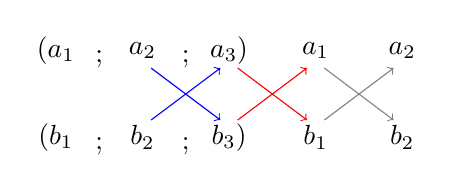
\begin{tikzpicture}[scale=1.1]


            \node at (0,1) {$(a_1$};
            \node at (0.5,0.9) {$;$};
            \node at (1,1) {$a_2$};
            \node at (1.5,0.9) {$;$};
            \node at (2,1) {$a_3)$};
            \node at (0,0) {$(b_1$};
            \node at (0.5,-0.1) {$;$};
            \node at (1,0) {$b_2$};
            \node at (1.5,-0.1) {$;$};
            \node at (2,0) {$b_3)$};
            \node at (3,1) {$a_1$};
            \node at (3,0) {$b_1$};
            \node at (4,1) {$a_2$};
            \node at (4,0) {$b_2$};


            % modré šipky
            \draw[->, blue] (1.1,0.8) -- (1.9,0.2);
            \draw[->, blue] (1.1,0.2) -- (1.9,0.8);

            % červené šipky
            \draw[->, red] (2.1,0.8) -- (2.9,0.2);
            \draw[->, red] (2.1,0.2) -- (2.9,0.8);

            % šedé šipky
            \draw[->, gray] (3.1,0.8) -- (3.9,0.2);
            \draw[->, gray] (3.1,0.2) -- (3.9,0.8);

        \end{tikzpicture}
        \caption{Pomůcka pro zapamatování vektorového součinu}
        \label{fig:cross_product_memory}
    \end{figure}
\end{remark}

Dále můžeme \textbf{vektorový součin} vektorů $\vec{u}$ a $\vec{v}$ vyjádřit pomocí vzorce pro velikost vektorového součinu a úhlu mezi těmito vektory.
Podobně jak jsme měli u skalárního součinu, tak i u vektorového součinu můžeme použít vzorec pro výpočet velikosti vektorového součinu pomocí úhlu mezi vektory.

\begin{definition}\label{def:cross_product_sin}
    Nechť $\vec{u}$ a $\vec{v}$ jsou vektory v prostoru a $\theta$ je úhel mezi těmito vektory. 
    Velikost vektorového součinu $\vec{u} \times \vec{v}$ je dána vztahem:
    \begin{equation}\label{eq:cross_product_sin}
        |\vec{u} \times \vec{v}| = |\vec{u}| \cdot |\vec{v}| \cdot \sin \theta.
    \end{equation}
    
\end{definition}

\begin{example}\label{exa:cross_product_of_vectors1}
    Vypočítejte vektorý součin vektorů $\vec{u} = (-2;1;3)$ a $\vec{v} = (1;2;3)$.
    Použijeme vzorec pro vektorový součin (\ref{eq:cross_product_space}):
    \begin{align*}
        \vec{u} \times \vec{v} &= (1 \cdot 3 - 3 \cdot 2;\, 3 \cdot 1 - (-2) \cdot 3;\, (-2) \cdot 2 - 1 \cdot 1)\\
                                &= (3 - 6;\, 3 + 6;\, -4 - 1)\\
                                &= (-3; 9; -5).
    \end{align*}
\end{example}

\begin{example}\label{exa:cross_product_of_vectors2}
    Vypočítejte vektorý součin vektorů $\vec{u} = (1;2;3)$ a $\vec{v} = (-2;1;3) $.
    Použijeme vzorec pro vektorový součin (\ref{eq:cross_product_space}):
    \begin{align*}
        \vec{u} \times \vec{v} &= (2 \cdot 3 - 3 \cdot 1;\, 3 \cdot (-2) - 1 \cdot 3;\, 1 \cdot 1 - 2 \cdot (-2))\\
                                &= (6 - 3;\, -6 - 3;\, 1 + 4)\\
                                &= (3; -9; 5).
    \end{align*}
\end{example}

Vnimněme si, že vektorový součin vektorů $\vec{u}$ a $\vec{v}$ z prvního příkladu (viz \ref{exa:cross_product_of_vectors1}) je roven opačnému vektoru vektorového součinu vektorů $\vec{v}$ a $\vec{u}$ z druhého příkladu (viz \ref{exa:cross_product_of_vectors2}):

\begin{example}
    Najděte vektor $\vec{w}$, který je kolmý k vektorům $\vec{u} = (1;0;1)$ a $\vec{v} = (1;2;2)$ a má velikost 6.
    Pro vektor $\vec{w}$, který je kolmý k vektorům $\vec{u}$ a $\vec{v}$, musí platit, že jeho směr je dán vektorovým součinem vektorů $\vec{u}$ a $\vec{v}$, a jeho velikost musí být rovna 6.
    Nejprve vypočítáme vektorový součin vektorů $\vec{u}$ a $\vec{v}$:
    \begin{align*}
        \vec{u} \times \vec{v} &= (0 \cdot 2 - 1 \cdot 2;\, 1 \cdot 1 - 1 \cdot 2;\, 1 \cdot 2 - 0 \cdot 1)\\
                                &= (0 - 2;\, 1 - 2;\, 2 - 0)\\
                                &= (-2; -1; 2).
    \end{align*}

    Nyní vypočítáme velikost vektoru $\vec{u} \times \vec{v}$:
    \[
        |\vec{u} \times \vec{v}| = \sqrt{(-2)^2 + (-1)^2 + 2^2} = \sqrt{4 + 1 + 4} = \sqrt{9} = 3.
    \]

    Vektor $\vec{w}$, který je kolmý k vektorům $\vec{u}$ a $\vec{v}$ a má velikost 6, můžeme získat násobením vektoru $\vec{u} \times \vec{v}$ skalárem $k$, kde $k$ je dán vzorcem:
    \[
        k = \frac{6}{|\vec{u} \times \vec{v}|} = \frac{6}{3} = 2.
    \]
    Nyní můžeme vypočítat vektor $\vec{w}$:
    \[
        \vec{w} = k \cdot (\vec{u} \times \vec{v}) = 2 \cdot (-2; -1; 2) = (-4; -2; 4).
    \]

    Tedy vektor $\vec{w} = (-4; -2; 4)$ je kolmý k vektorům $\vec{u}$ a $\vec{v}$ a má velikost 6.
    Případně vektor $\vec{w} = (4; 2; -4)$ je také kolmý k vektorům $\vec{u}$ a $\vec{v}$ a má velikost 6, protože je roven opačnému vektoru $\vec{w}$.
\end{example}


Pomocí vektorového součinu můžeme také vypočítat obsah trojúhelníka, 
který je určen třemi body v prostoru.

\begin{example}\label{exa:cross_product_area_parallelogram}
    Mějme body $A[-1; -2; 1]$, $B[2;0;2]$ a $C[1;1;-1]$. Určete obsah čtyřúhelníka $ABCD$.

    Nejprve si ujasníme, co vlastně počítáme. Body $A$, $B$ a $C$ určují dva vektory,
    které mají společný počátek v bodě $A$. Tyto dva vektory tvoří strany rovnoběžníku $ABCD$.

    Obsah tohoto rovnoběžníku tedy můžeme určit pomocí těchto dvou vektorů.

    Využijeme vztah pro velikost vektorového součinu:
    \[
    |\vec{u} \times \vec{v}| = |\vec{u}| \cdot |\vec{v}| \cdot \sin\varphi,
    \]
    kde $\varphi$ je úhel mezi vektory $\vec{u}$ a $\vec{v}$.

    Zároveň víme ze základní geometrie, že obsah rovnoběžníku se stranami délky $a$ a $b$ a úhlem $\alpha$ je
    \[
    S = a \cdot b \cdot \sin\alpha.
    \]

    Porovnáním těchto dvou vztahů vidíme, že obsah rovnoběžníku je roven velikosti vektorového součinu:
    \[
    S = |\vec{u} \times \vec{v}|.
    \]

    Nyní si tedy vytvoříme vektory, které odpovídají stranám rovnoběžníku:
    \begin{align*}
        \vec{u} &= \overrightarrow{AB} = (2 - (-1);\; 0 - (-2);\; 2 - 1) = (3;\, 2;\, 1),\\
        \vec{v} &= \overrightarrow{AC} = (1 - (-1);\; 1 - (-2);\; -1 - 1) = (2;\, 3;\, -2).
    \end{align*}

    Nyní vypočítáme vektorový součin $\vec{u} \times \vec{v}$.
    Použijeme determinantový vzorec (resp. pravidlo pro složky):

    \begin{align*}
        \vec{u} \times \vec{v}  &= (u_2 v_3 - u_3 v_2;\; u_3 v_1 - u_1 v_3;\; u_1 v_2 - u_2 v_1) \\
                                &= (2 \cdot (-2) - 1 \cdot 3;\; 1 \cdot 2 - 3 \cdot (-2);\; 3 \cdot 3 - 2 \cdot 2) \\
                                &= (-4 - 3;\; 2 + 6;\; 9 - 4) \\
                                &= (-7;\, 8;\, 5).
    \end{align*}

    Nás zajímá velikost tohoto vektoru, protože ta odpovídá obsahu rovnoběžníku:
    \begin{align*}
    |\vec{u} \times \vec{v}|    &= \sqrt{(-7)^2 + 8^2 + 5^2} \\
                                &= \sqrt{49 + 64 + 25} \\
                                &= \sqrt{138} \approx 11{,}75.
    \end{align*}

    Obsah čtyřúhelníka $ABCD$ (rovnoběžníku) je tedy přibližně $11{,}75$.
\end{example}


\begin{example}\label{exa:cross_product_volume_of_parallelepiped}
    Jsou dány body $A[1;0;1]$, $B[3;-1;4]$, $D[2;2;2]$ a $E[-1;3;5]$. Určete objem rovnoběžnostěnu ABCDEFGH.

    Nejprve si ujasníme, jak budeme postupovat. Rovnoběžnostěn je určen třemi vektory,
    které vycházejí ze stejného bodu (zde z bodu $A$).

    Tyto vektory odpovídají hranám (stranám) rovnoběžnostěnu, které vycházejí z bodu $A$ (viz obrázek~\ref{fig:parallelepiped_abcde}):
    \[
    \vec{u} = \overrightarrow{AB}, \quad
    \vec{v} = \overrightarrow{AD}, \quad
    \vec{w} = \overrightarrow{AE}.
    \]
    
    \begin{figure}[H]
        \centering
        \begin{tikzpicture}[scale=1]

            % Body a roviny
            \coordinate (A) at (0,0,2);
            \fill (A) circle (2pt);
            \node[below right] at (A) {$A$};
            \coordinate (B) at (4,0,2);
            \fill (B) circle (2pt);
            \node[below right] at (B) {$B$};
            \coordinate (D) at (0,0,0);
            \fill (D) circle (2pt);
            \node[below right] at (D) {$D$};
            \coordinate (E) at (0.5,2,2);
            \fill (E) circle (2pt);
            \node[below right] at (E) {$E$};
            \coordinate (C) at (4,0,0);
            \fill (C) circle (2pt);
            \node[below right] at (C) {$C$};
            \coordinate (F) at (4.5,2,2);
            \fill (F) circle (2pt);
            \node[below right] at (F) {$F$};
            \coordinate (G) at (4.5,2,0);
            \fill (G) circle (2pt);
            \node[below right] at (G) {$G$};
            \coordinate (H) at (0.5,2,0);
            \fill (H) circle (2pt);
            \node[below right] at (H) {$H$};

            % rovnoběžnostěn
            \draw[fill=blue!30, opacity=0.2] (A) -- (B) -- (C) -- (D) -- cycle;
            \draw[fill=blue!30, opacity=0.2] (A) -- (B) -- (F) -- (E) -- cycle;
            \draw[fill=blue!30, opacity=0.2] (A) -- (D) -- (H) -- (E) -- cycle;
            \draw[fill=blue!30, opacity=0.2] (B) -- (C) -- (G) -- (F) -- cycle;
            \draw[fill=blue!30, opacity=0.2] (D) -- (C) -- (G) -- (H) -- cycle;
            \draw[fill=blue!30, opacity=0.2] (E) -- (F) -- (G) -- (H) -- cycle;

            % vektory
            \draw[vector] (A) -- (B) node[above, midway, sloped] {$\vec{u}$};
            \draw[vector] (A) -- (D) node[above, midway, sloped] {$\vec{v}$};
            \draw[vector] (A) -- (E) node[above, midway, sloped] {$\vec{w}$};
        \end{tikzpicture}
        \caption{Rovnoběžnostěn ABCDEFGH}
        \label{fig:parallelepiped_abcde}
    \end{figure}

    Objem rovnoběžnostěnu je dán tzv. smíšeným součinem:
    \[
    V = |\vec{u} \cdot (\vec{v} \times \vec{w})|.
    \]

    Geometricky tento vztah říká:
    \begin{itemize}
        \item $\vec{v} \times \vec{w}$ určuje obsah podstavy (rovnoběžníku),
        \item skalární součin s $\vec{u}$ „přidá výšku“.
    \end{itemize}

    Nejprve tedy určíme jednotlivé vektory:
    \begin{align*}
    \vec{u} &= \overrightarrow{AB} = (3 - 1;\; -1 - 0;\; 4 - 1) = (2;\, -1;\, 3),\\
    \vec{v} &= \overrightarrow{AD} = (2 - 1;\; 2 - 0;\; 2 - 1) = (1;\, 2;\, 1),\\
    \vec{w} &= \overrightarrow{AE} = (-1 - 1;\; 3 - 0;\; 5 - 1) = (-2;\, 3;\, 4).
    \end{align*}

    Nyní vypočítáme vektorový součin $\vec{v} \times \vec{w}$:
    \begin{align*}
    \vec{v} \times \vec{w}
    &= (2 \cdot 4 - 1 \cdot 3;\; 1 \cdot (-2) - 1 \cdot 4;\; 1 \cdot 3 - 2 \cdot (-2)) \\
    &= (8 - 3;\; -2 - 4;\; 3 + 4) \\
    &= (5;\, -6;\, 7).
    \end{align*}

    Tento vektor reprezentuje obsah podstavy (včetně směru).

    Nyní provedeme skalární součin s vektorem $\vec{u}$:
    \begin{align*}
    \vec{u} \cdot (\vec{v} \times \vec{w})
    &= (2;\, -1;\, 3) \cdot (5;\, -6;\, 7) \\
    &= 2 \cdot 5 + (-1) \cdot (-6) + 3 \cdot 7 \\
    &= 10 + 6 + 21 \\
    &= 37.
    \end{align*}

    Objem musí být nezáporný, proto bereme absolutní hodnotu:
    \[
    V = 37.
    \]

    Tento výraz nazýváme \textbf{smíšený součin} vektorů $\vec{u}$, $\vec{v}$ a $\vec{w}$.


\end{example}


\subsubsection{Smíšený součin}\label{subsubsec:Complex_cross_dot_product_in_space}
Tímto příkladem (viz příklad \ref{exa:cross_product_volume_of_parallelepiped}) jsme si ukázali, jak můžeme využít vektorový součin pro výpočet objemu rovnoběžnostěnu,
a zároveň jsme si ukázali, že vektorový součin je důležitým nástrojem pro řešení mnoha geometrických problémů v prostoru,
a že nám umožňuje vypočítat nejen obsah rovnoběžníku, ale i objem rovnoběžnostěnu a dalších geometrických útvarů v prostoru.

\begin{definition}\label{def:scalar_triple_product}
    Nechť $\vec{u}$, $\vec{v}$ a $\vec{w}$ jsou vektory v prostoru. 
    \textbf{Smíšený součin} vektorů $\vec{u}$, $\vec{v}$ a $\vec{w}$ je definován jako:
    \begin{equation}\label{eq:scalar_triple_product}
        \vec{u} \cdot (\vec{v} \times \vec{w}).
    \end{equation}
\end{definition}

\textbf{Smíšený součin} vektorů $\vec{u}$, $\vec{v}$ a $\vec{w}$ nám dává číslo, které reprezentuje objem rovnoběžnostěnu určeného těmito třemi vektory.
Smíšený součin tedy vzniká tak, že nejprve vypočítáme vektorový součin dvou vektorů (například $\vec{v} \times \vec{w}$), a poté provedeme skalární součin tohoto výsledného vektoru s třetím vektorem.
Geometricky tento vztah říká, že \textbf{vektorový součin určuje obsah podstavy rovnoběžníku}, a \textbf{skalární součin s třetím vektorem určuje výšku}.
Smíšený součin je důležitým nástrojem pro řešení mnoha geometrických problémů v prostoru, a umožňuje nám vypočítat objem rovnoběžnostěnu a dalších geometrických útvarů v prostoru.

Smíšený součin spojuje oba předchozí součiny (skalární a vektorový) s již známými geometrickými vztahy (obsah rovnoběžníku a objem rovnoběžnostěnu), a umožňuje nám tak řešit komplexní geometrické problémy v prostoru pomocí jednoduchých algebraických operací s vektory.
\begin{align*}
    \text{vektorový součin} \quad &\rightarrow \quad \text{obsah rovnoběžníku} \\
    \text{skalární součin} \quad &\rightarrow \quad \text{projekce (výška)} \\
    \textbf{smíšený součin} \quad &\rightarrow \quad \text{objem rovnoběžnostěnu}
\end{align*}

\begin{remark}
    Smíšený součin úzce souvisí s determinantem matice řádu $3 \times 3$.

    Konkrétně platí, že výraz
    \[
    \vec{u} \cdot (\vec{v} \times \vec{w})
    \]
    lze zapsat jako \textbf{determinant matice} složené ze souřadnic těchto vektorů:
    \[
    \vec{u} \cdot (\vec{v} \times \vec{w})
    =
    \begin{vmatrix}
        u_1 & u_2 & u_3 \\
        v_1 & v_2 & v_3 \\
        w_1 & w_2 & w_3
    \end{vmatrix}.
    \]

    Tento zápis si blíže vysvětlíte v lineární algebře, se kterou se setkáte na vysoké škole.
\end{remark}







